\section{Results}
\label{chap:results}

This section presents and discusses our achieved results, considering the described metrics and experimental protocol. The results of our proposal are compared to state-of-the-art methods. Results regarding the developed mobile application are presented alongside visual examples.

\subsection{Comparisons with Baselines}

This section presents the experimental results of the proposed method (MobText) and a comparison with the state-of-the-art methods for text localization. Table~\ref{tab:comparison-efficacy-deep-learning-methods-icdar11} shows the results for the evaluated methods considering the ICDAR'11 dataset. In this case, the MobText method achieved the best results with Precision, Recall, and F-measure values of $97.40\%$, $94.81\%$, and $96.09\%$, respectively. On the other hand, the SqueezeDet network presented the lowest Precision and F-measure among the evaluated methods ($56.36\%$ and $66.01\%$, respectively). In turn, the TextBoxes achieved the lowest results of Recall ($71.93\%$).
%
\begin{table}[!h]
    \centering
    \caption{Comparison of effectiveness among the evaluated deep learning-based methods for the ICDAR'11 dataset.}
    \label{tab:comparison-efficacy-deep-learning-methods-icdar11}
    \resizebox{0.9\columnwidth}{!}{ 
    \begin{tabular}{lrrr}
        \topline
        \headcol
        \textbf{Methods}       & \textbf{Precision (\%)} &  \textbf{Recall (\%)} &  \textbf{F-measure (\%)} \\ 
        \midline
        MobText        & \highlight{97.40} & \highlight{94.81} & \highlight{96.09} \\ \hline
         SSTD                   & $89.28$           & $78.53$           & $83.56$           \\ \hline
         TextBoxes              & $92.15$           & $71.93$           & $80.80$           \\ \hline
         TextBoxes++            & $95.76$           & $90.51$           & $93.06$           \\ \hline
         YOLOv3                 & $94.27$           & $89.21$           & $91.67$           \\ \hline
         SqueezeDet             & $56.36$           & $79.66$           & $66.01$           \\
       \bottomlinec
    \end{tabular}}
\end{table}

With regard to ICDAR'13 dataset, the SSTD methods presented the highest Recall ($82.19\%$), and F-measure ($86.33\%$), while the YOLOv3 reached the best results in terms of Precision (Table~\ref{tab:comparison-efficacy-deep-learning-methods-icdar13}). Note, however, that the MobText yields very competitive results for this dataset as well, in terms of Precision. 
%In contrast, the SqueezeDet presented the lowest Precision, Recall, and F-measure, with values about $29.41\%$, $62.47\%$, and $39.99\%$, respectively.
%
\begin{table}[!h]
    \centering
    \caption{Comparison of effectiveness among the evaluated deep learning-based methods for the ICDAR'13 dataset.}
    \label{tab:comparison-efficacy-deep-learning-methods-icdar13}
    \resizebox{0.9\columnwidth}{!}{ 
    \begin{tabular}{lrrr}
        \topline
        \headcol
        \textbf{Methods}       & \textbf{Precision (\%)} &  \textbf{Recall (\%)} &  \textbf{F-measure (\%)} \\ 
        \midline
        MobText        & $88.04$           & $63.20$           & $73.58$           \\ \hline
        TextBoxes++            & $90.49$           & $80.82$           & $85.38$           \\ \hline
         SSTD                   & {90.91} & \highlight{82.19} & \highlight{86.33} \\ \hline
         TextBoxes              & $88.84$           & $74.16$           & $80.83$           \\ \hline
         YOLOv3                 & \highlight{92.01}           & $75.71$           & $83.07$           \\ \hline
         SqueezeDet             & $29.41$           & $62.47$           & $39.99$           \\ 
       \bottomlinec
    \end{tabular}}
\end{table}
%
\begin{figure}[!h]
    \centering
    % 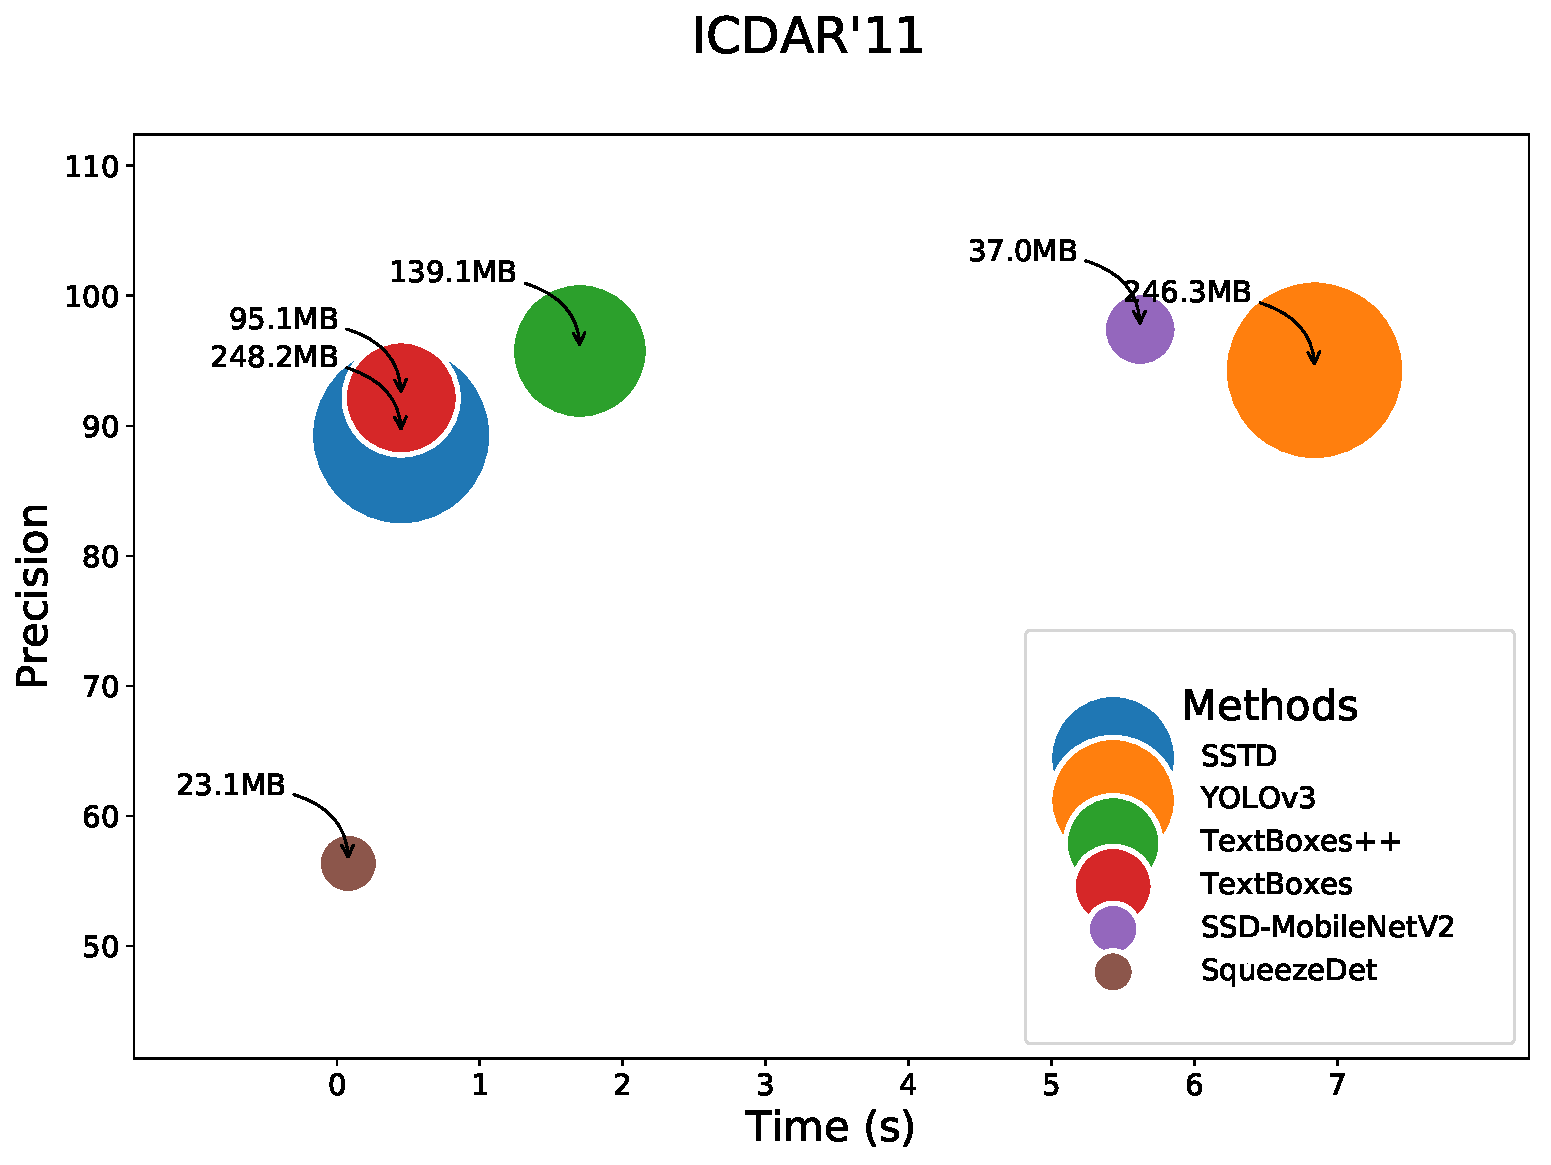
\includegraphics[height=0.25\textheight]{VISAPP/figs/efficacy-and-efficiency/deep-methods-icdar11-precision.pdf}
    % 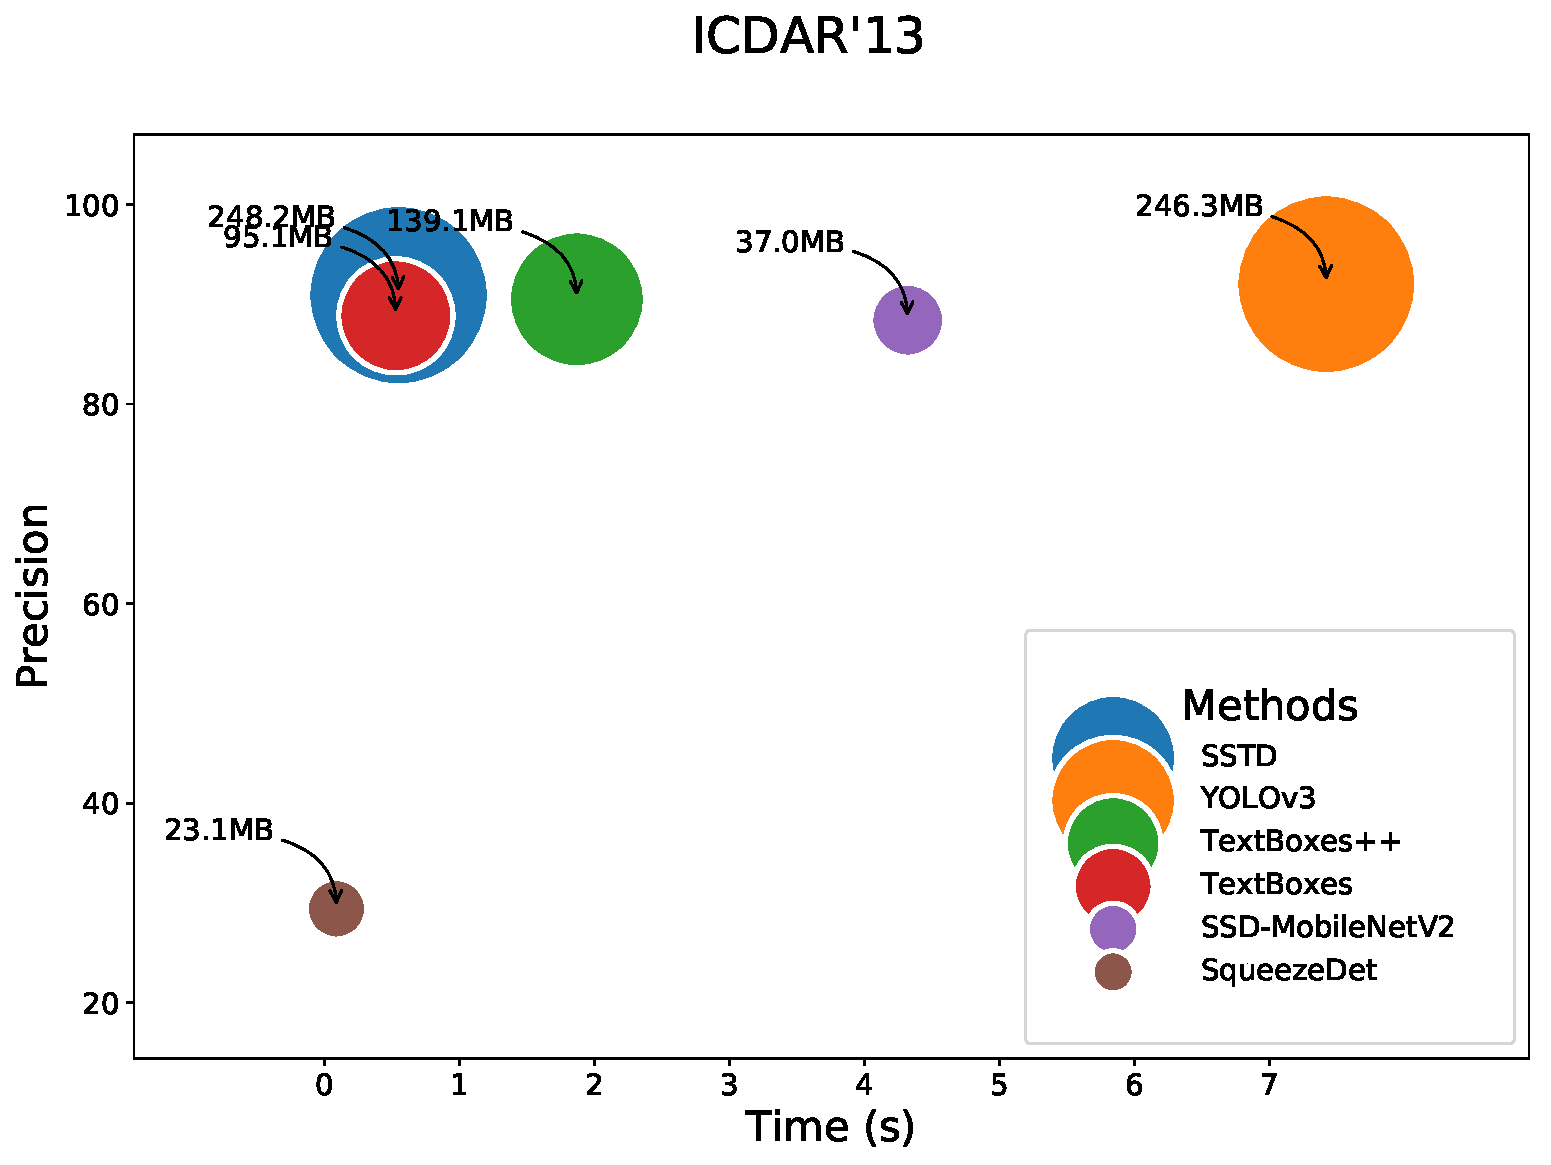
\includegraphics[height=0.25\textheight]{VISAPP/figs/efficacy-and-efficiency/deep-methods-icdar13-precision.pdf} \\
    % 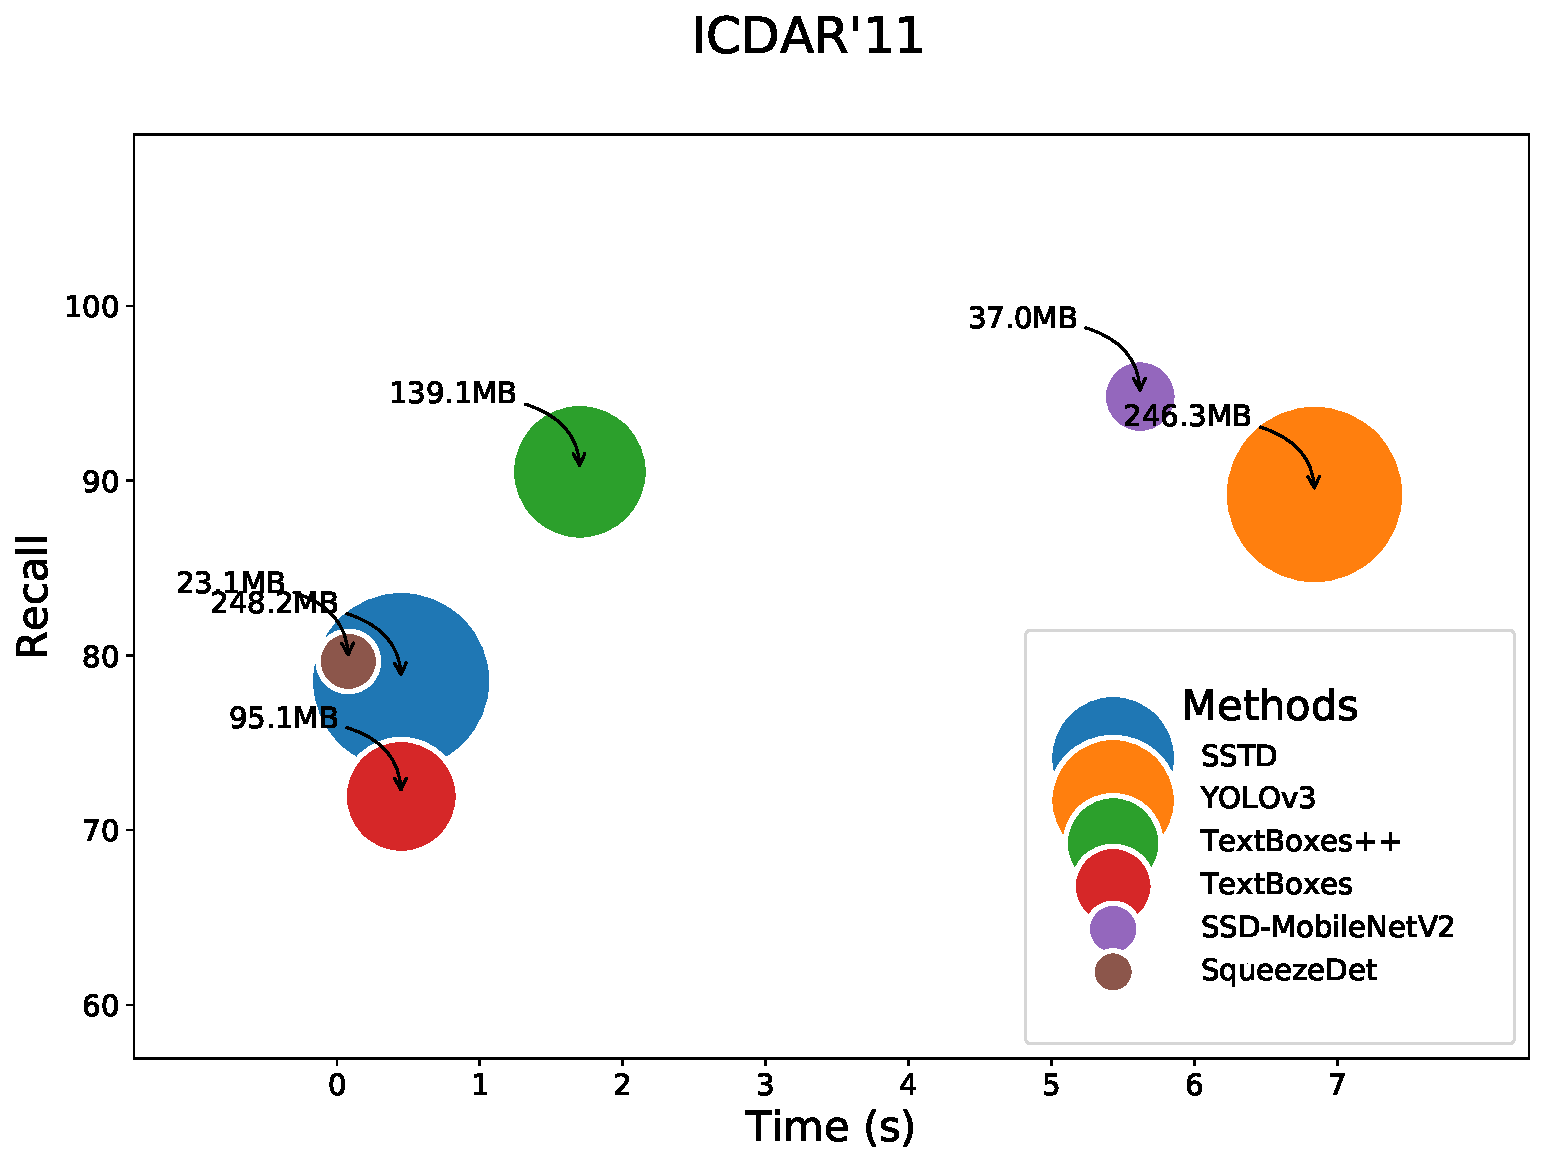
\includegraphics[height=0.25\textheight]{figs/efficacy-and-efficiency/deep-methods-icdar11-recall.pdf}
    % 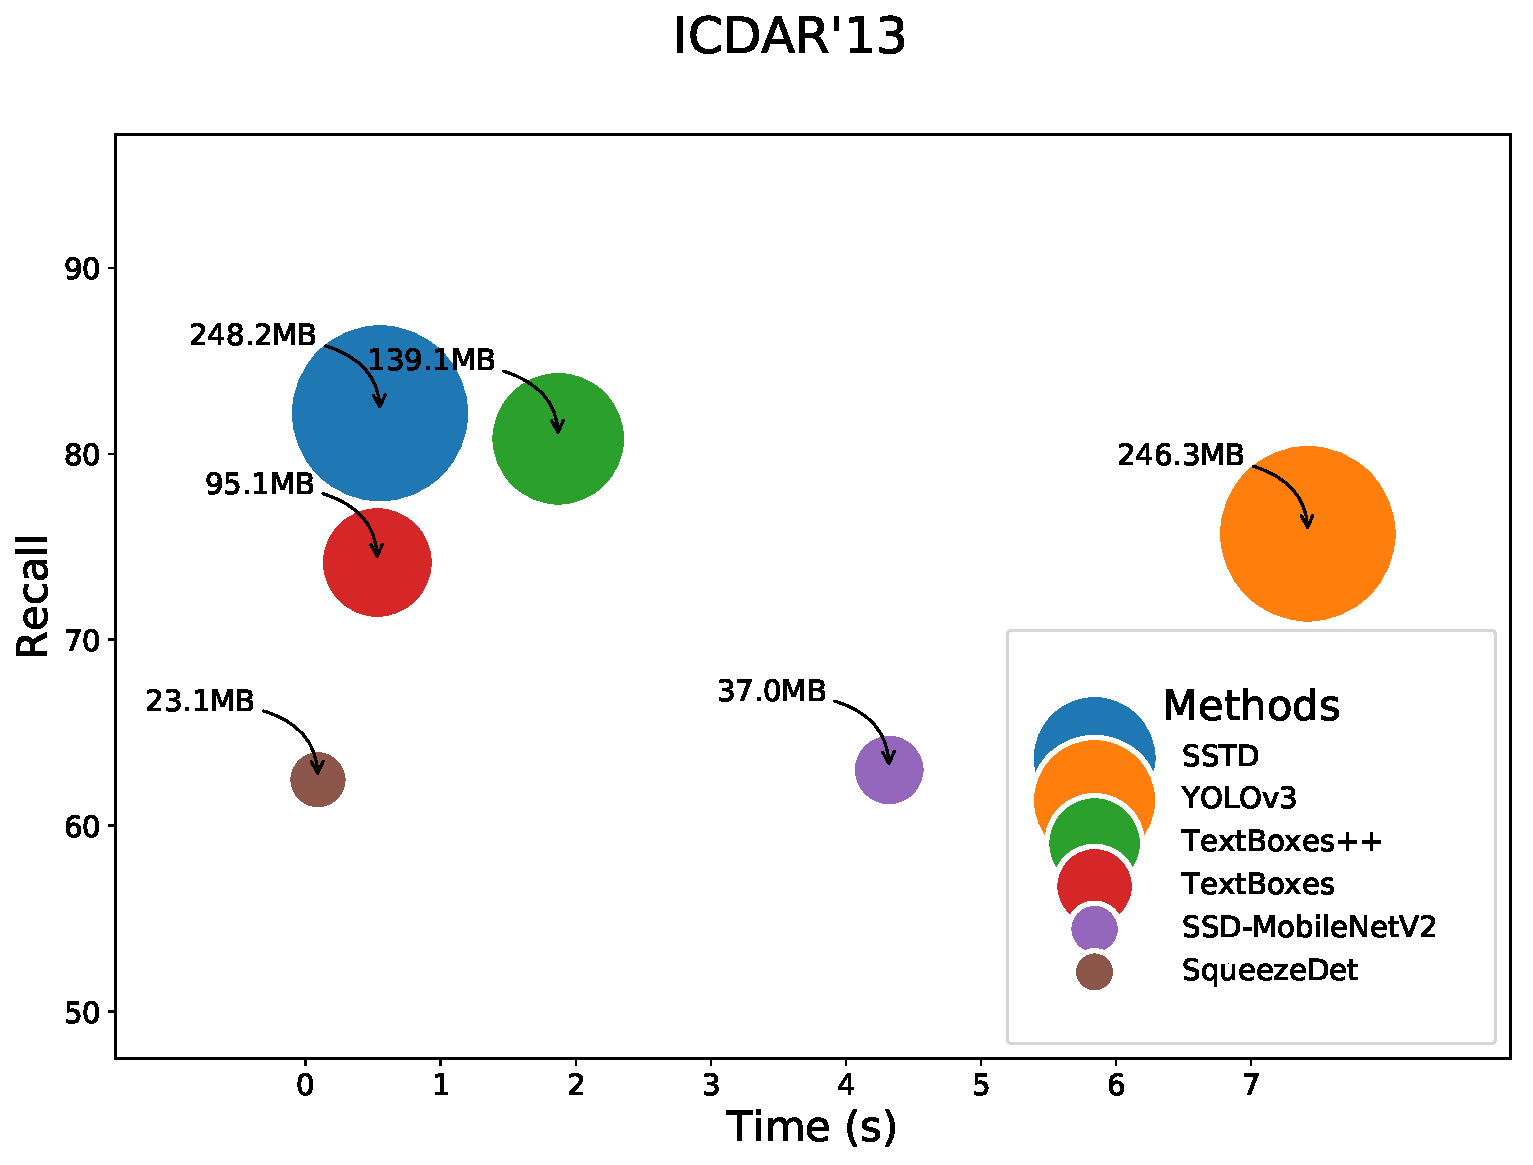
\includegraphics[height=0.25\textheight]{figs/efficacy-and-efficiency/deep-methods-icdar13-recall.pdf} \\
    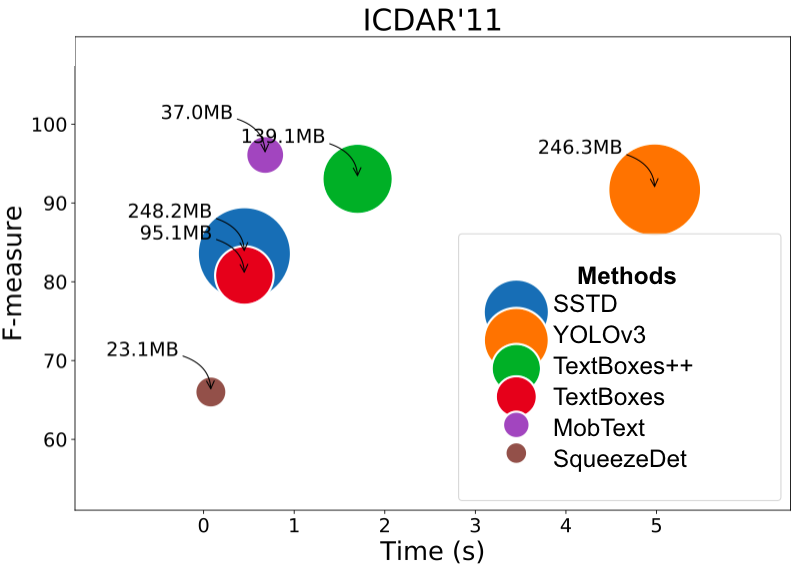
\includegraphics[width=0.80\textwidth]{ICIP_frankenstein/figs/deep-methods-icdar11-f-measure.png} \\
    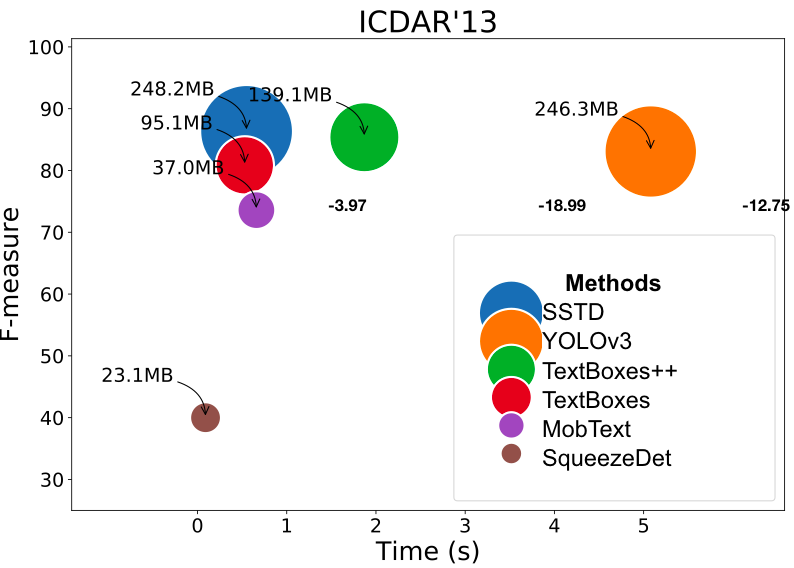
\includegraphics[width=0.80\textwidth]{ICIP_frankenstein/figs/deep-methods-icdar13-f-measure.png}
    \caption{Comparison results among the evaluated methods considering aspects of efficacy and efficiency.}
    \label{fig:deep-methods-efficacy-and-efficiency}
\end{figure}

%Now, we will turn our attention for 
In term of 
%evaluating 
the efficiency of the presented methods, 
Fig.~\ref{fig:deep-methods-efficacy-and-efficiency} summarizes the results considering the metrics used to assess the effectiveness of the evaluated methods, in terms of F-measure, along with the metrics for measuring the efficiency of those methods, considering the ICDAR'11 and ICDAR'13 datasets.

Regarding efficiency (processing time and disk usage), the proposed method (MobText) yielded very competitive results, taking only $0.45$ and $0.55$ seconds per image, considering the ICDAR'11 and ICDAR'13, respectively. Comparing MobText with the baseline methods originally proposed for text localization (TextBoxes, TextBoxes++, SSTD), the proposed method presented very competitive results with a processing time of $0.67$ seconds per image and with disk usage of about $37.0$MB. In contrast, the most effective baseline methods, the SSTD and TextBoxes++ networks, presented competitive results in terms of effectiveness and worse results in terms of processing time in comparison with the proposed method. Regarding the disk usage, MobText also presented the best balance between accuracy and model size.   

Now, when compared with the state-of-the-art approaches for object detection, the proposed method also presented competitive results. In this case, the fastest approach for text localization was the SqueezeDet network, which takes about $0.1$ seconds per image, on average. However, when we take into account the trade-off between efficiency and effectiveness, we can safely argue that the proposed method presented a better compromise between these two measures. Figure~\ref{fig:qualitative-results-good-11} provides some cases of success and Figure~\ref{fig:qualitative-results-bad-11} cases of failure of the proposed method for the ICDAR'11 and Figures~\ref{fig:qualitative-results-good-13} and~\ref{fig:qualitative-results-bad-13} for ICDAR'13 datasets. 


\begin{figure}[!h]
	\centering

    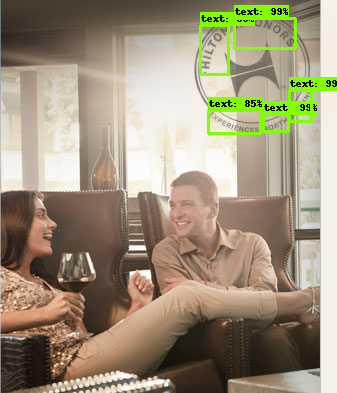
\includegraphics[height=0.29\textheight]{VISAPP/figs/qualitative-results/icdar11/69.png}
    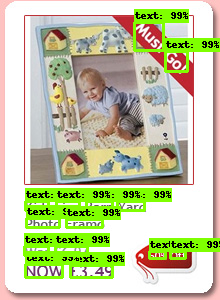
\includegraphics[height=0.29\textheight]{VISAPP/figs/qualitative-results/icdar11/46.png}
    
    \vspace{1.5mm}
    
    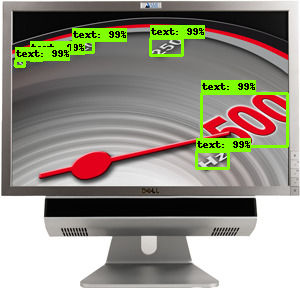
\includegraphics[height=0.20\textheight]{VISAPP/figs/qualitative-results/icdar11/14.png}
    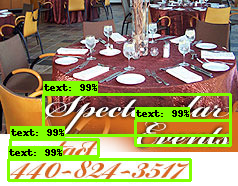
\includegraphics[height=0.20\textheight]{VISAPP/figs/qualitative-results/icdar11/29.png}
    
    \caption{Examples of success cases of the proposed approach for the ICDAR'11 dataset. Green bounding boxes indicate the regions correctly localized.}
	\label{fig:qualitative-results-good-11}
\end{figure}

%includegraphics[width=0.19\textwidth]{VISAPP/figs/qualitative-results/icdar11/117.png} \\

\begin{figure}[!h]
	\centering

    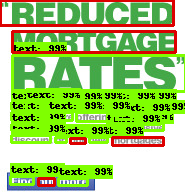
\includegraphics[height=0.20\textheight]{VISAPP/figs/qualitative-results/icdar11/22m.png}
    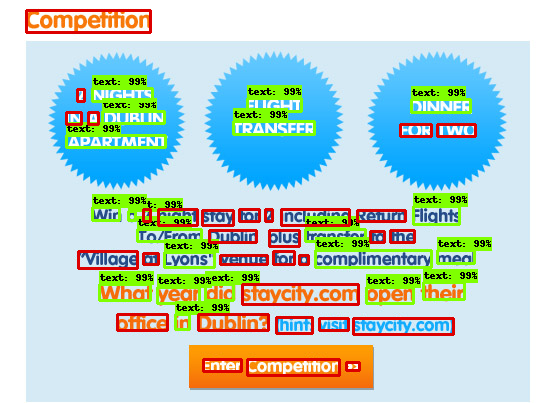
\includegraphics[height=0.20\textheight]{VISAPP/figs/qualitative-results/icdar11/53m.png}

    \vspace{1.5mm}

    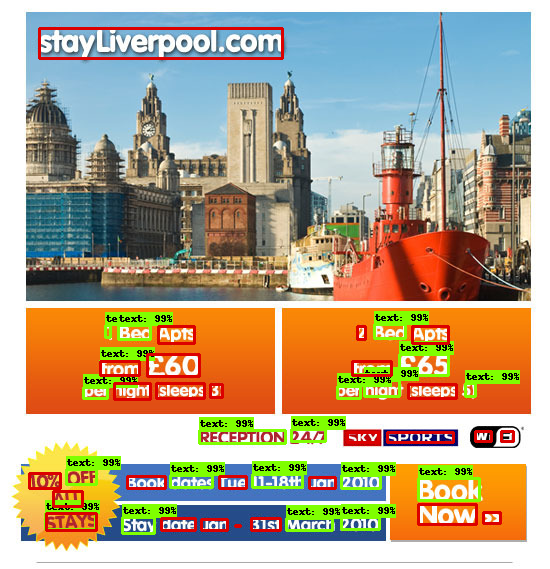
\includegraphics[height=0.25\textheight]{VISAPP/figs/qualitative-results/icdar11/32m.png}
    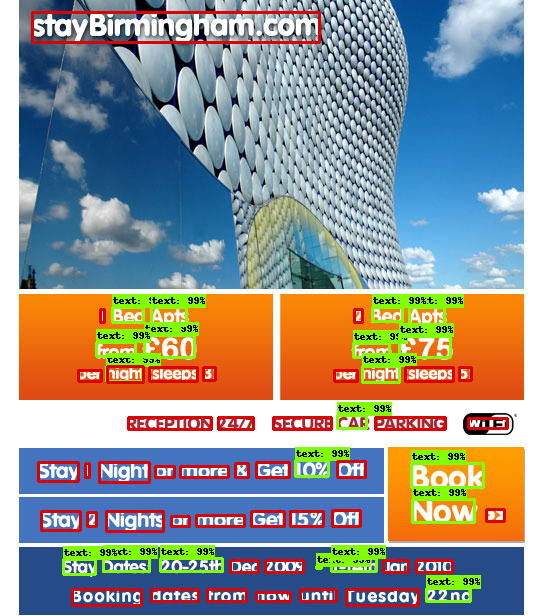
\includegraphics[height=0.25\textheight]{VISAPP/figs/qualitative-results/icdar11/10m.png}

\caption{Examples of failure cases of the proposed approach for the ICDAR'11 dataset. Green bounding boxes indicate the regions correctly localized, while red bounding boxes show candidate regions not detected by our method.}
	\label{fig:qualitative-results-bad-11}
\end{figure}

\begin{figure}[!h]
	\centering

    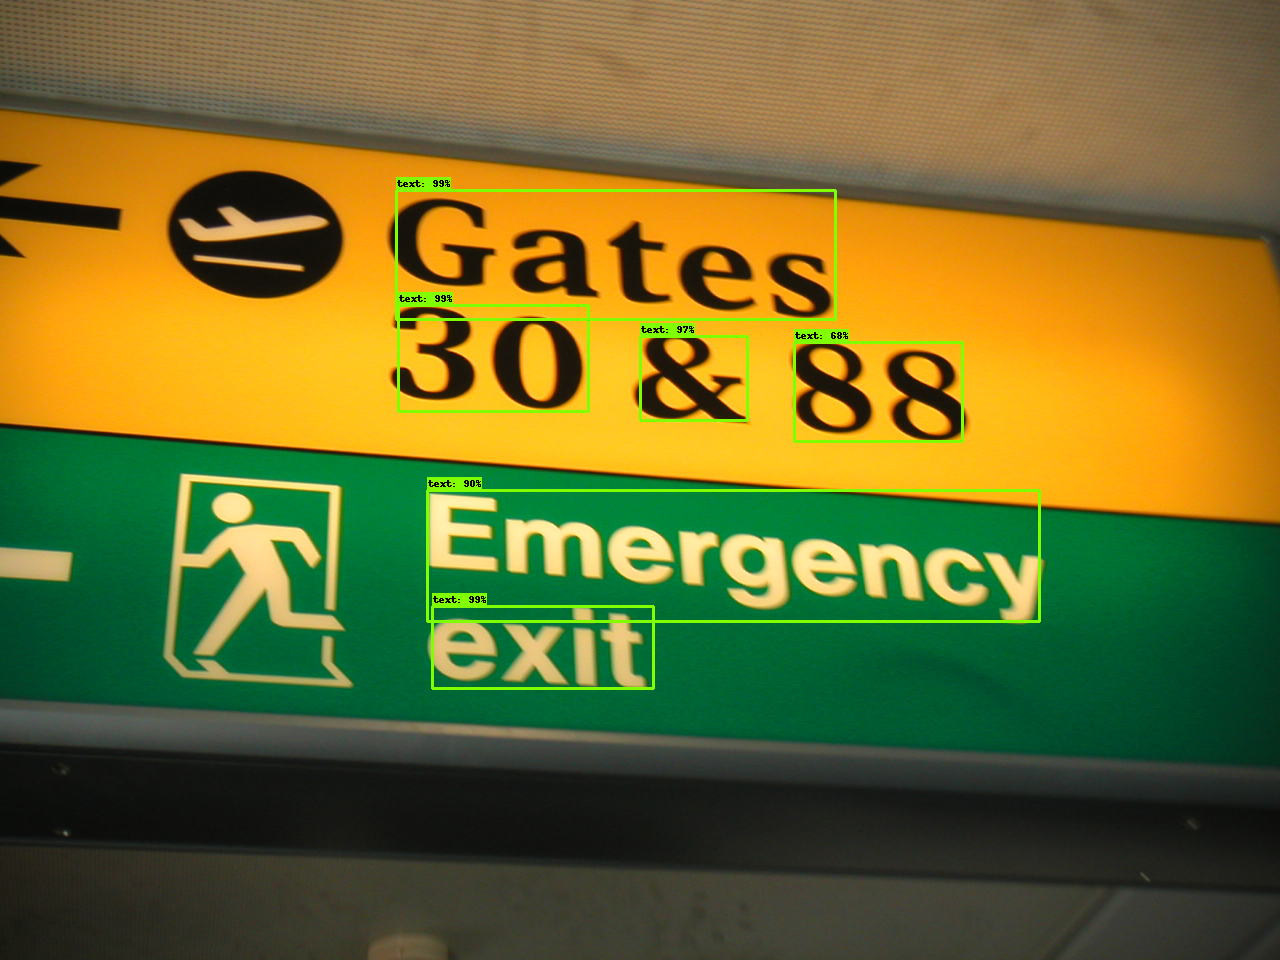
\includegraphics[height=0.20\textheight]{VISAPP/figs/qualitative-results/icdar13/19.png}
    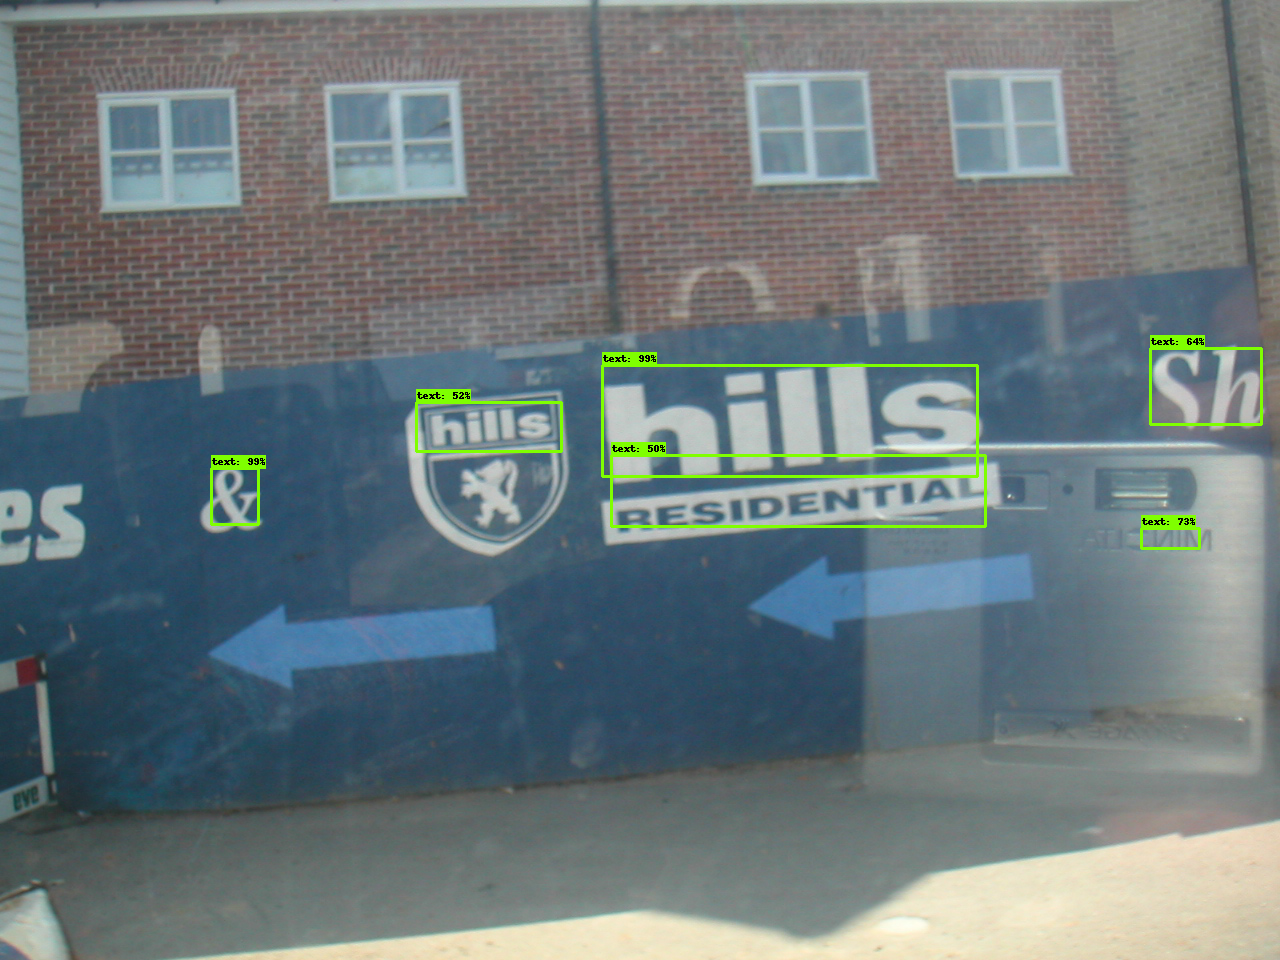
\includegraphics[height=0.20\textheight]{VISAPP/figs/qualitative-results/icdar13/83.png}
    
    \vspace{1.5mm}
    
    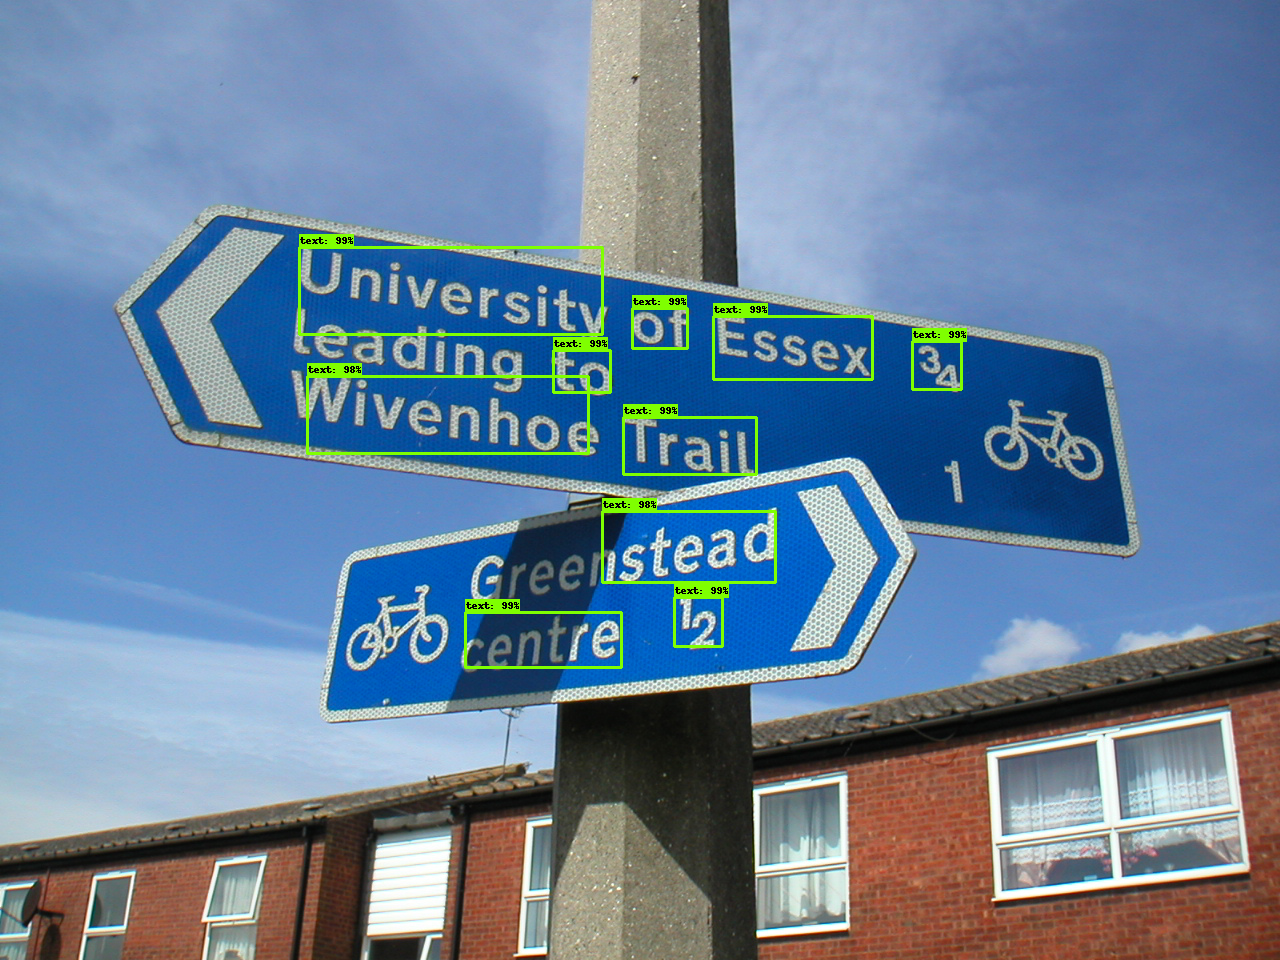
\includegraphics[height=0.20\textheight]{VISAPP/figs/qualitative-results/icdar13/129.png}
    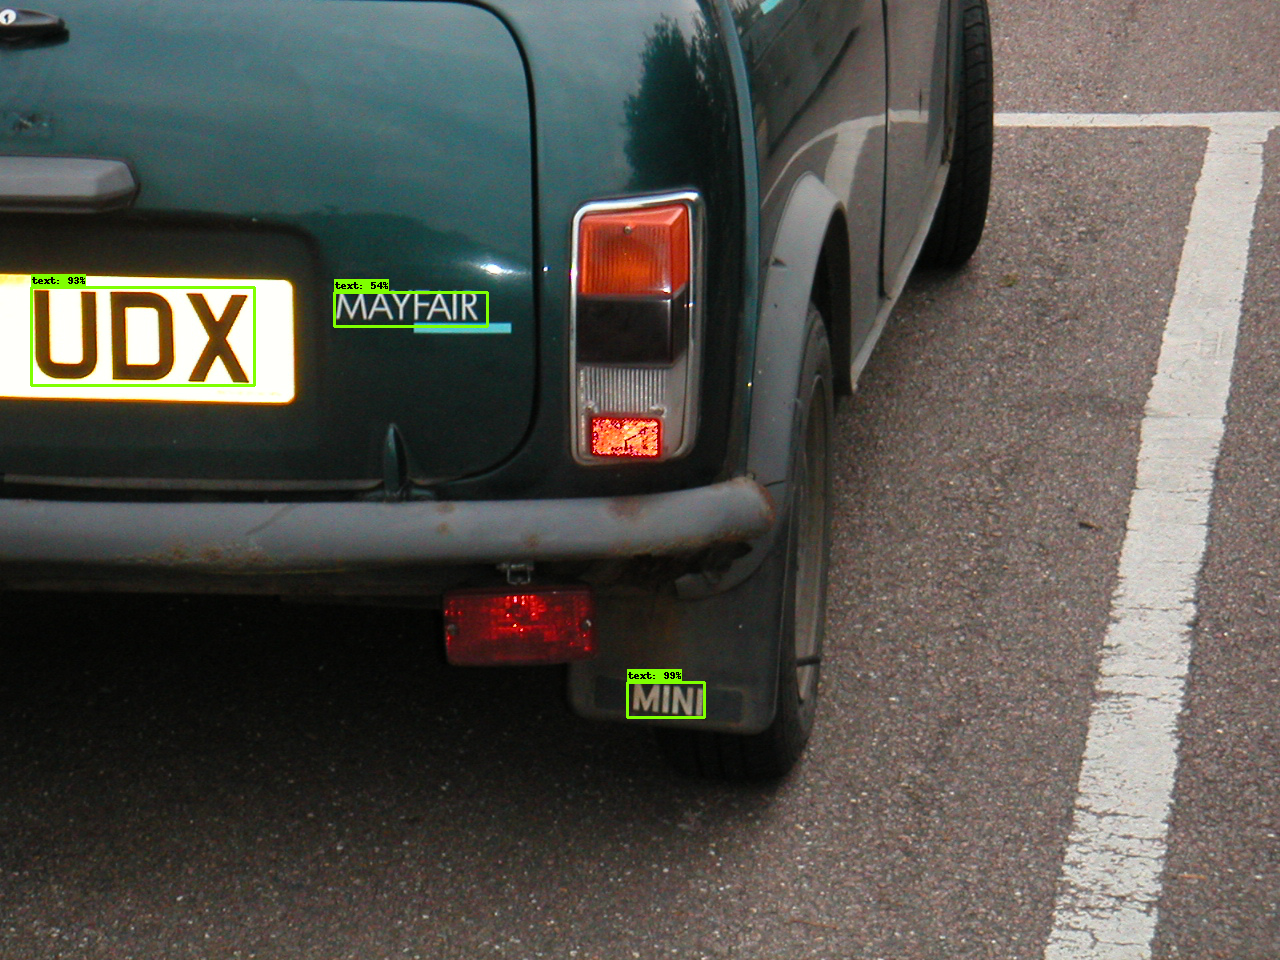
\includegraphics[height=0.20\textheight]{VISAPP/figs/qualitative-results/icdar13/140.png}
	\caption{Examples of success cases of the proposed approach for the ICDAR'13 dataset. Green bounding boxes indicate the regions correctly localized.}
	\label{fig:qualitative-results-good-13}
\end{figure}
\begin{figure}[!h]
	\centering
    
    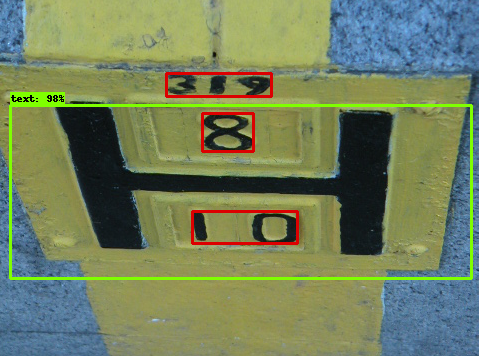
\includegraphics[height=0.20\textheight]{VISAPP/figs/qualitative-results/icdar13/1m_crop.png}
    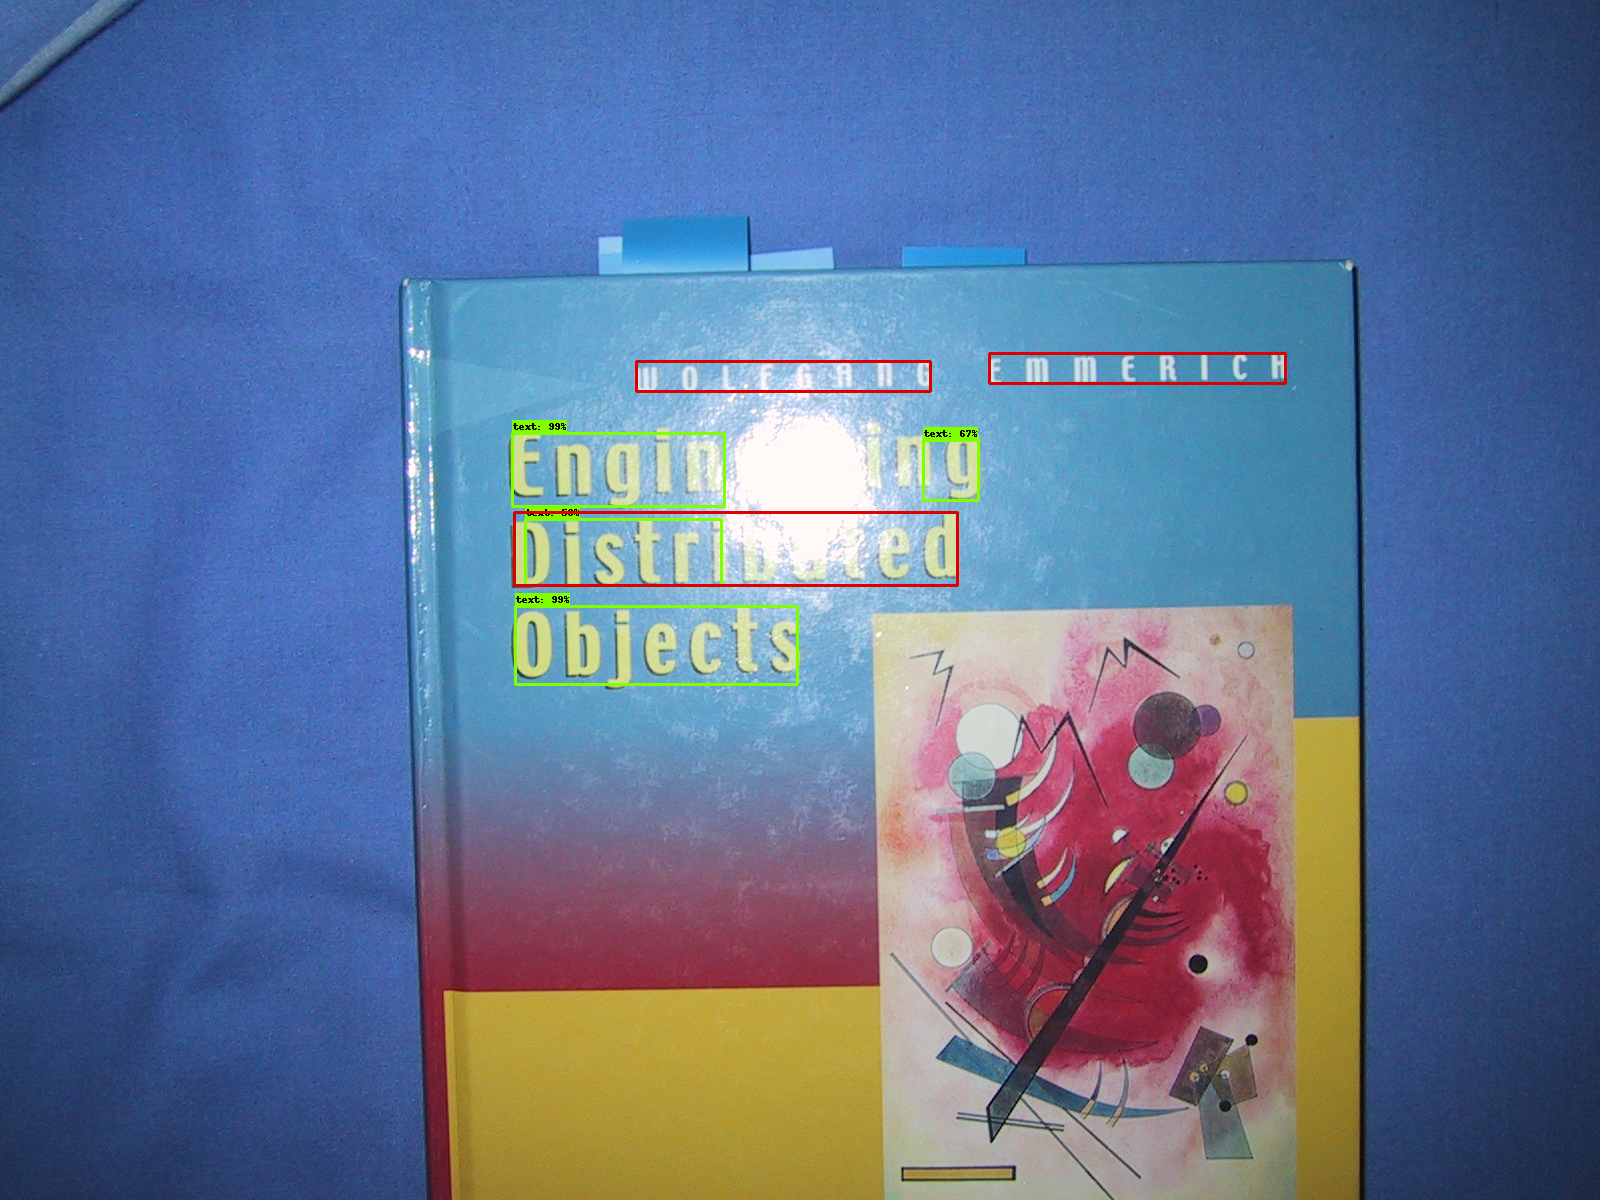
\includegraphics[height=0.20\textheight]{VISAPP/figs/qualitative-results/icdar13/18m.png}

    \vspace{1.5mm}

    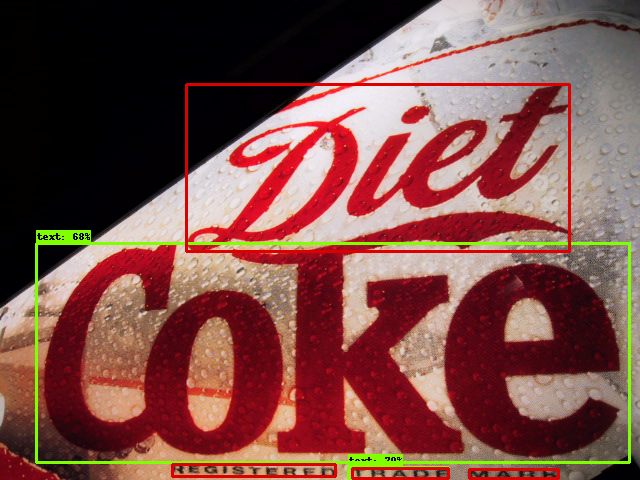
\includegraphics[height=0.20\textheight]{VISAPP/figs/qualitative-results/icdar13/41m.png}
    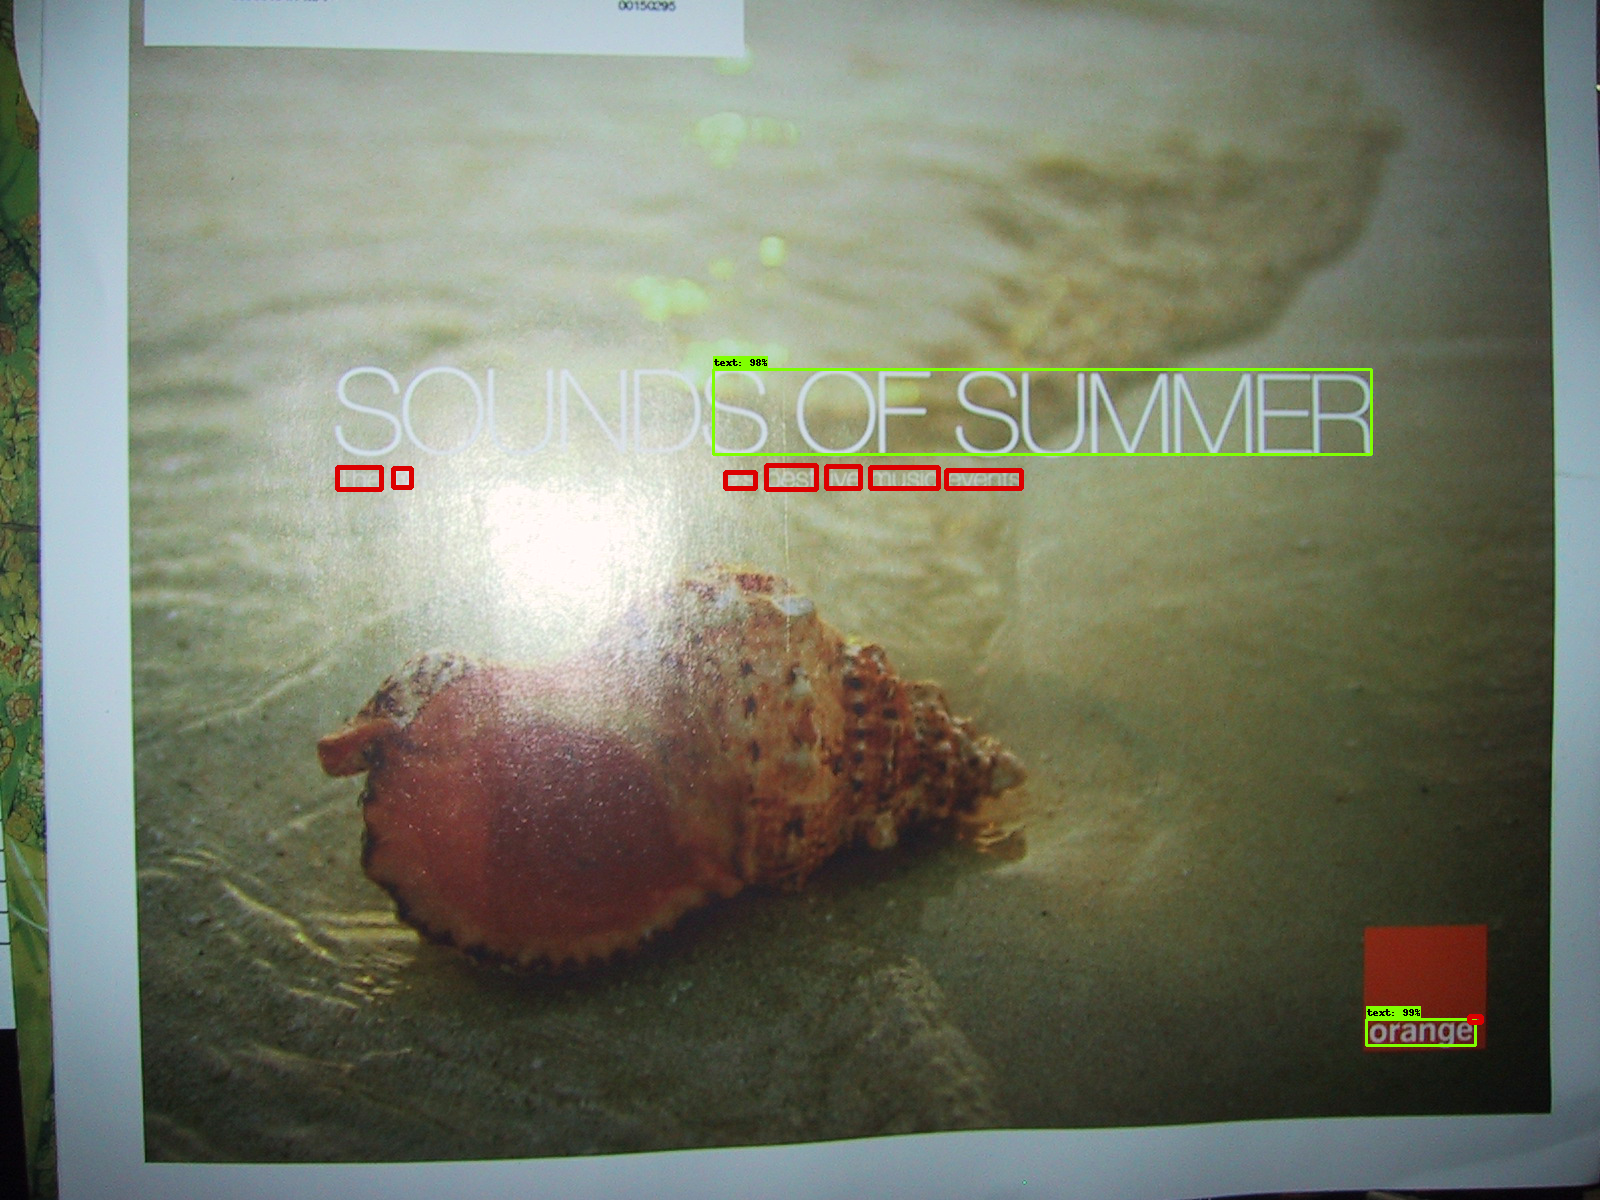
\includegraphics[height=0.20\textheight]{VISAPP/figs/qualitative-results/icdar13/48m.png}
%   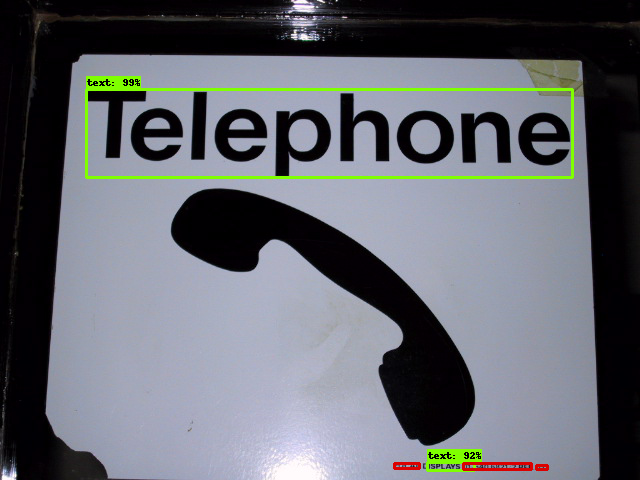
\includegraphics[height=0.20\textheight]{VISAPP/figs/qualitative-results/icdar13/49m.png}

	\caption{Examples of failure cases of the proposed approach for the ICDAR'13 dataset. Green bounding boxes indicate the regions correctly localized, while red bounding boxes show candidate regions were not detected by our method.}
	\label{fig:qualitative-results-bad-13}
\end{figure}

The proposed method is able to detect multi-oriented texts and even texts with textured backgrounds. However, as we could observe, the proposed approach presented some difficulties in localizing scene text in the ICDAR'13 dataset. In comparison with results achieved for the ICDAR'11, the precision and recall rates decreased $9.36$ and $31.61$ percentage points, respectively, which suggest that our network did not localized several candidate regions containing texts.

\begin{figure}[!h]
    \centering
    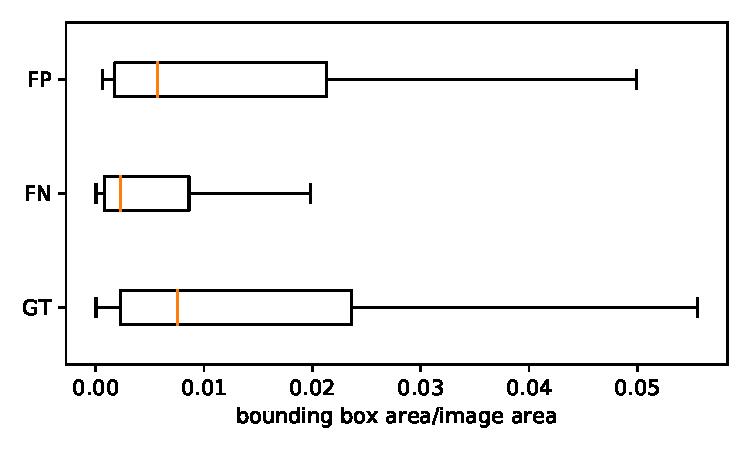
\includegraphics[width=0.75\textwidth]{VISAPP/figs/boxplot_error_icdar13.pdf}
    \caption{Comparison among distributions of relative areas of bounding boxes from Ground-Truth (GT), False Negatives (FN) cases, and False Positive (FP) cases. We omitted the points considered outliers for a better visualization.}
    \label{fig:boxplot}
\end{figure}

To understand the reasons that led the proposed method to have this difficult in localizing text for the ICDAR'13 datasets, we performed an analysis of failure cases taking into account the relative area of missed bounding boxes. Figure~\ref{fig:boxplot} presents a box-plot graph that shows the distribution of the relative area of bounding boxes (i.e., ratio of bounding box area to image area) for the ground-truth, false positive cases, and false negative cases.

\begin{figure}[!h]
    \centering
    %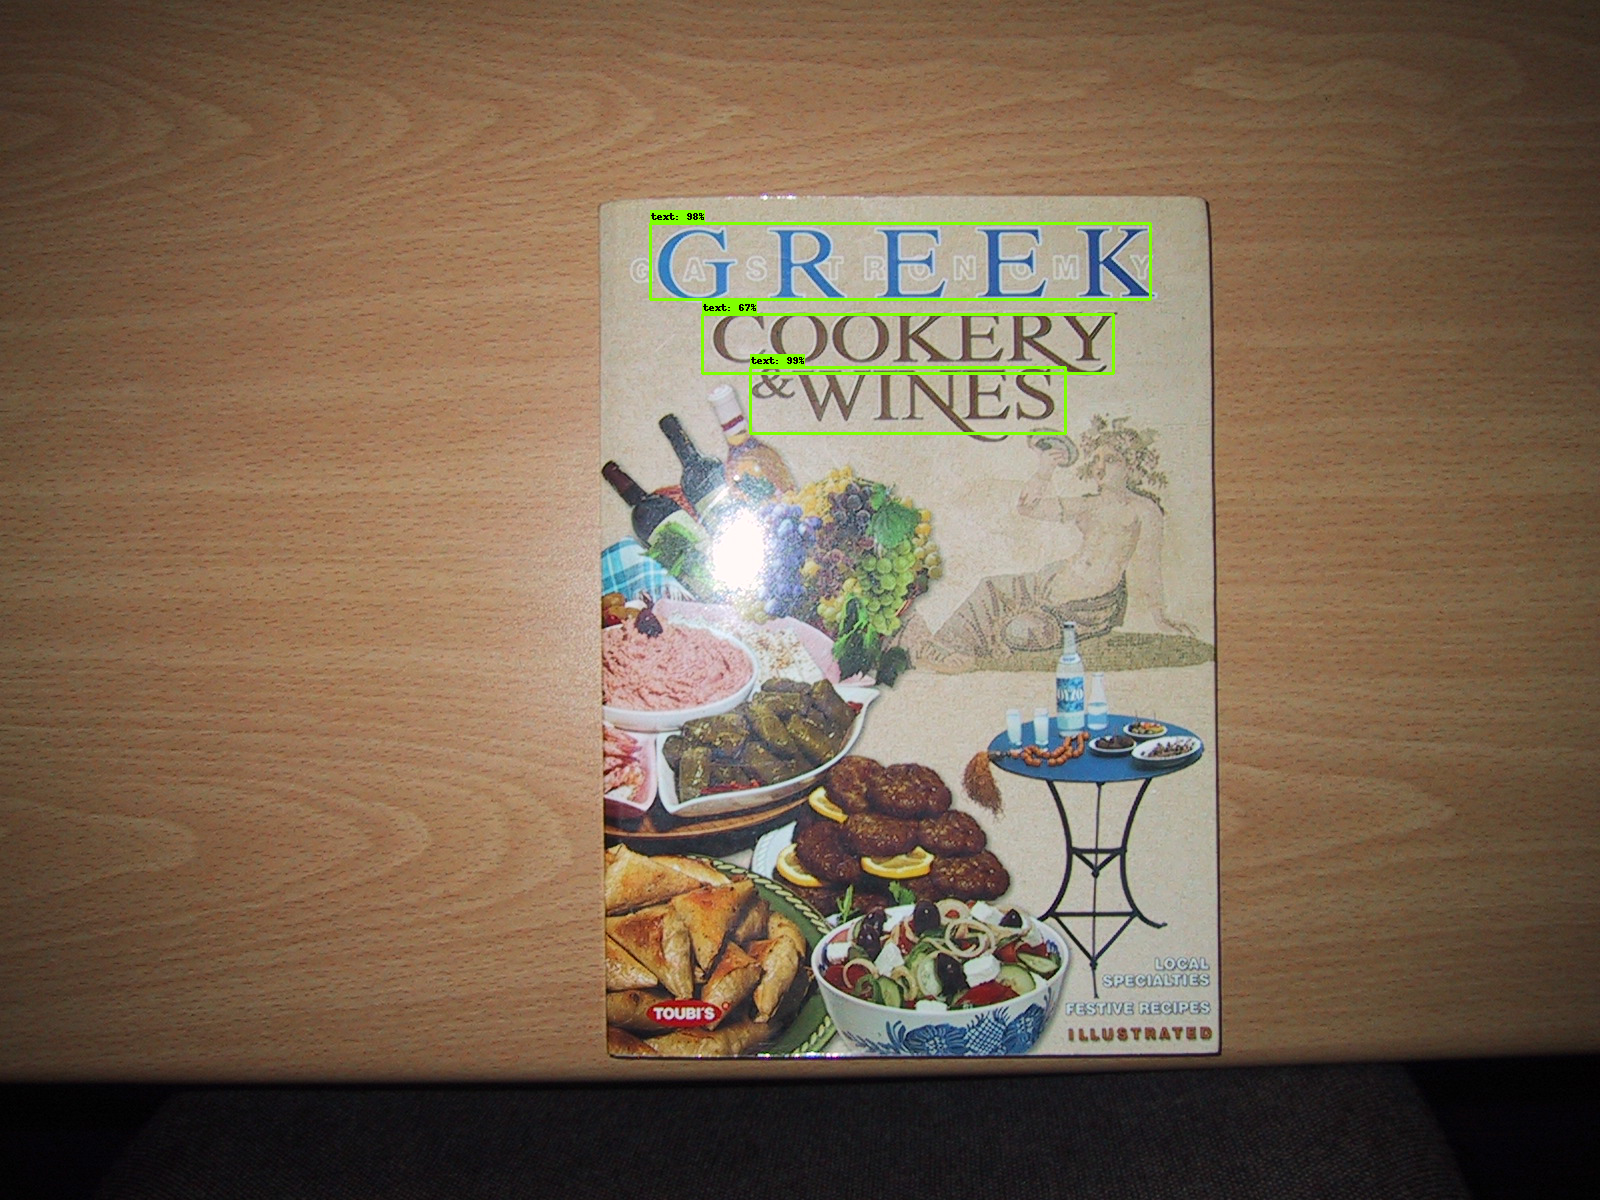
\includegraphics[width=\columnwidth]{version-2/figs/small_box.jpg}
    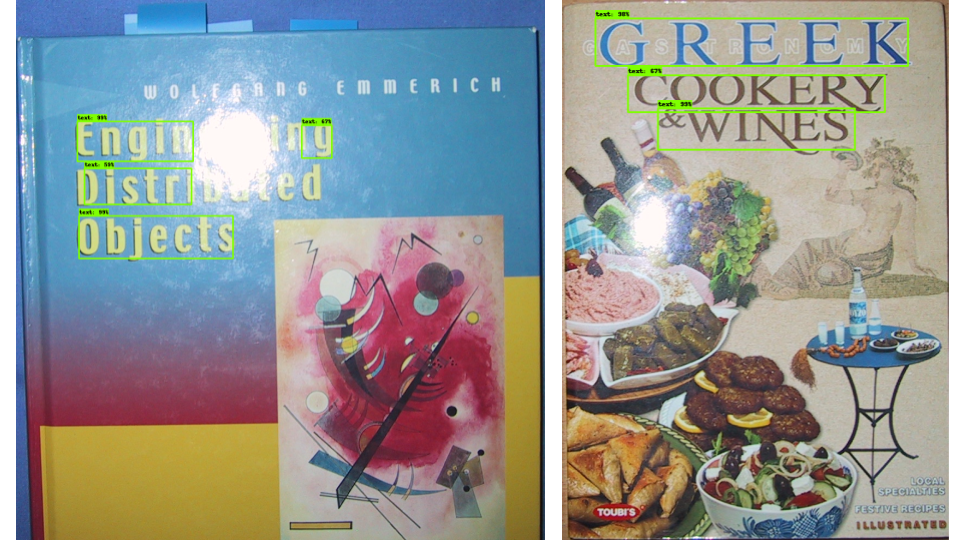
\includegraphics[width=0.99\textwidth]{VISAPP/figs/hires_samples.png}
    \caption{Two high resolution examples of ICDAR'13 dataset with both medium-sized text (detected by our method) and small-sized (not detected).}
    \label{fig:small_example}
\end{figure}

As we can observe, the missed bounding boxes (false negative cases) have a small relative area. More precisely, $75\%$ of false negative cases (third quartile of FN box-plot) have a relative area up to $0.01$ and correspond to $50\%$ of the bounding box present in the ground-truth (median of GT box-plot). This results suggest to us that high resolution images with relatively small text (see Fig.~\ref{fig:small_example}) are specially challenging to our method. To overcome this limitation, future investigations can be conducted to devise an architecture to better localize bounding boxes with multiple scales such as Feature Pyramid Networks (FPNs), as proposed by \citep{Lin2017CVPR}.

\subsection{Results on Mobile-Oriented Environment}

In terms of precision, recall, and F-Measure on ICDAR'11 and ICDAR'13 datasets, the proposal achieved the same results as on the non-restrictive scenario. Table~\ref{tab:times_dataset} shows the efficiency of the network in terms of inference time on both datasets. 

\begin{table}[!h]
    \centering
    \caption{Processing time of the embedded application on ICDAR datasets.}
    \label{tab:times_dataset}
    \begin{tabular}{lrrr}
        \toprule
        \ml{2}{*}{\textbf{Dataset}} & \mcol{3}{c}{\textbf{Processing Time (ms)}}  \\ 
                                    & \textbf{Min.} &  \textbf{Max.} &  \textbf{Average} \\ 
        \midrule
        ICDAR'11                    & $420$         & $524$          & $464$           \\ \hline
        ICDAR'13                    & $449$         & $602$          & $523$           \\
        
       \bottomrule
    \end{tabular}
\end{table}

As we are unable to evaluate the method in a quantitative manner regarding effectiveness on the images captured in the wild, the proposed solution was only evaluated in terms of efficiency, in processing time. A qualitative analysis was performed by taking into account the visual results of the detection on the images. 

 The average time of inference in $250$ images was $425$ms, with a minimum inference time of $343$ms and a maximum of $584$ms.


%%%%%%%%%%%%%%%%%
\begin{figure}[h!]
\centering
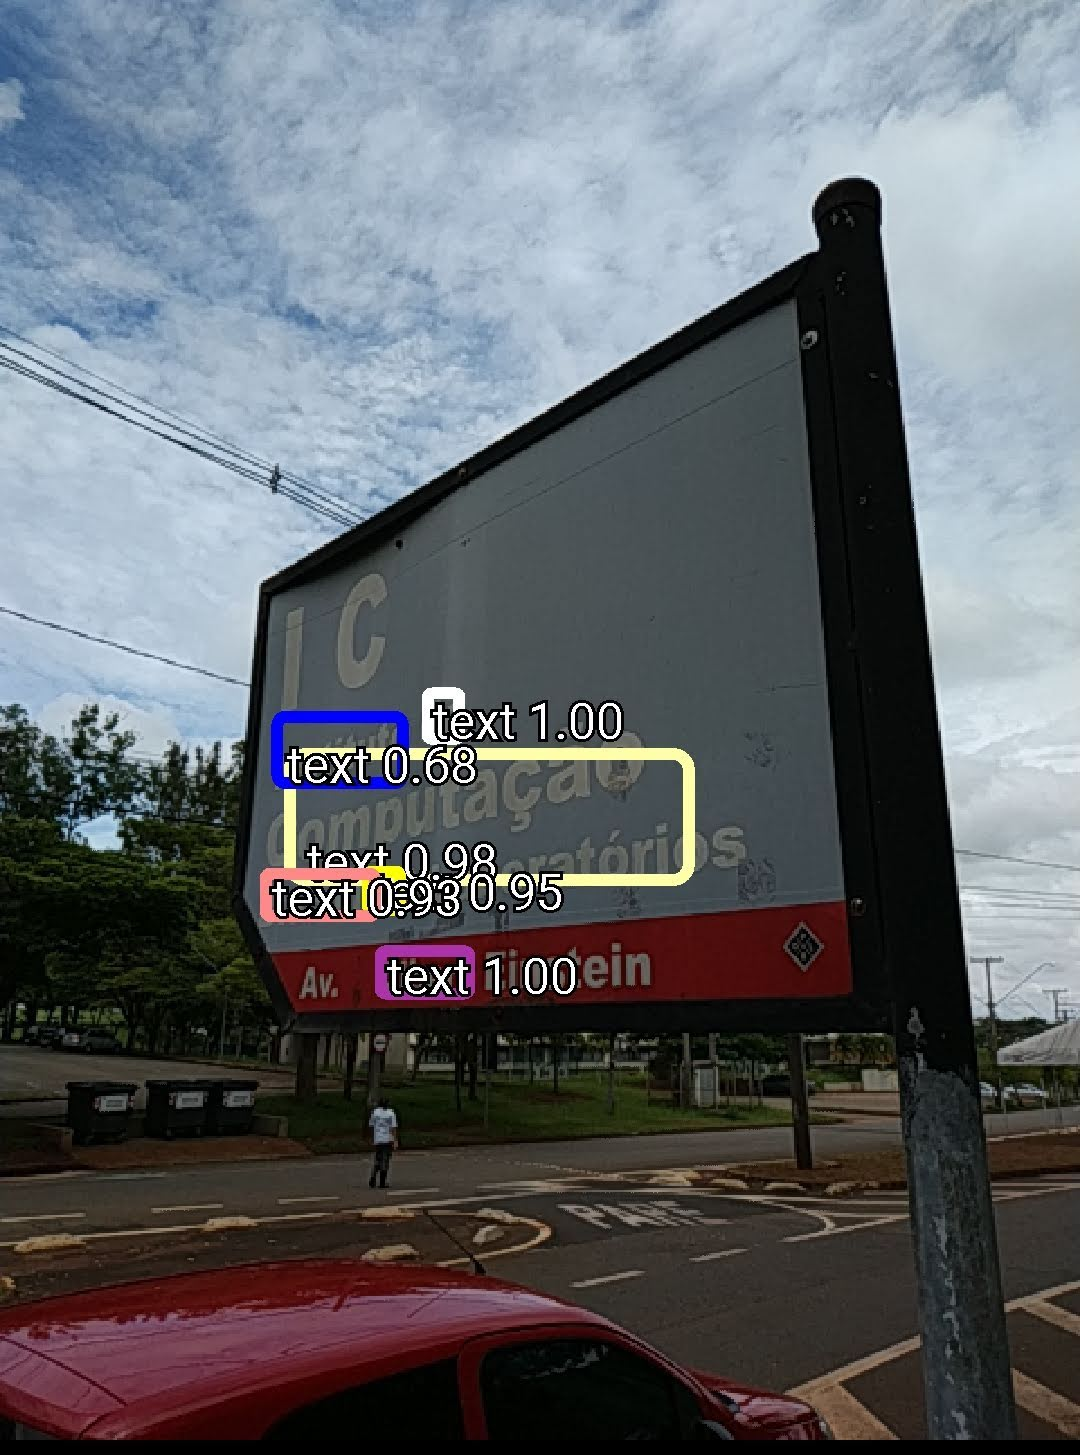
\includegraphics[width=0.49\textwidth]{Mobile/images/app27.jpg}
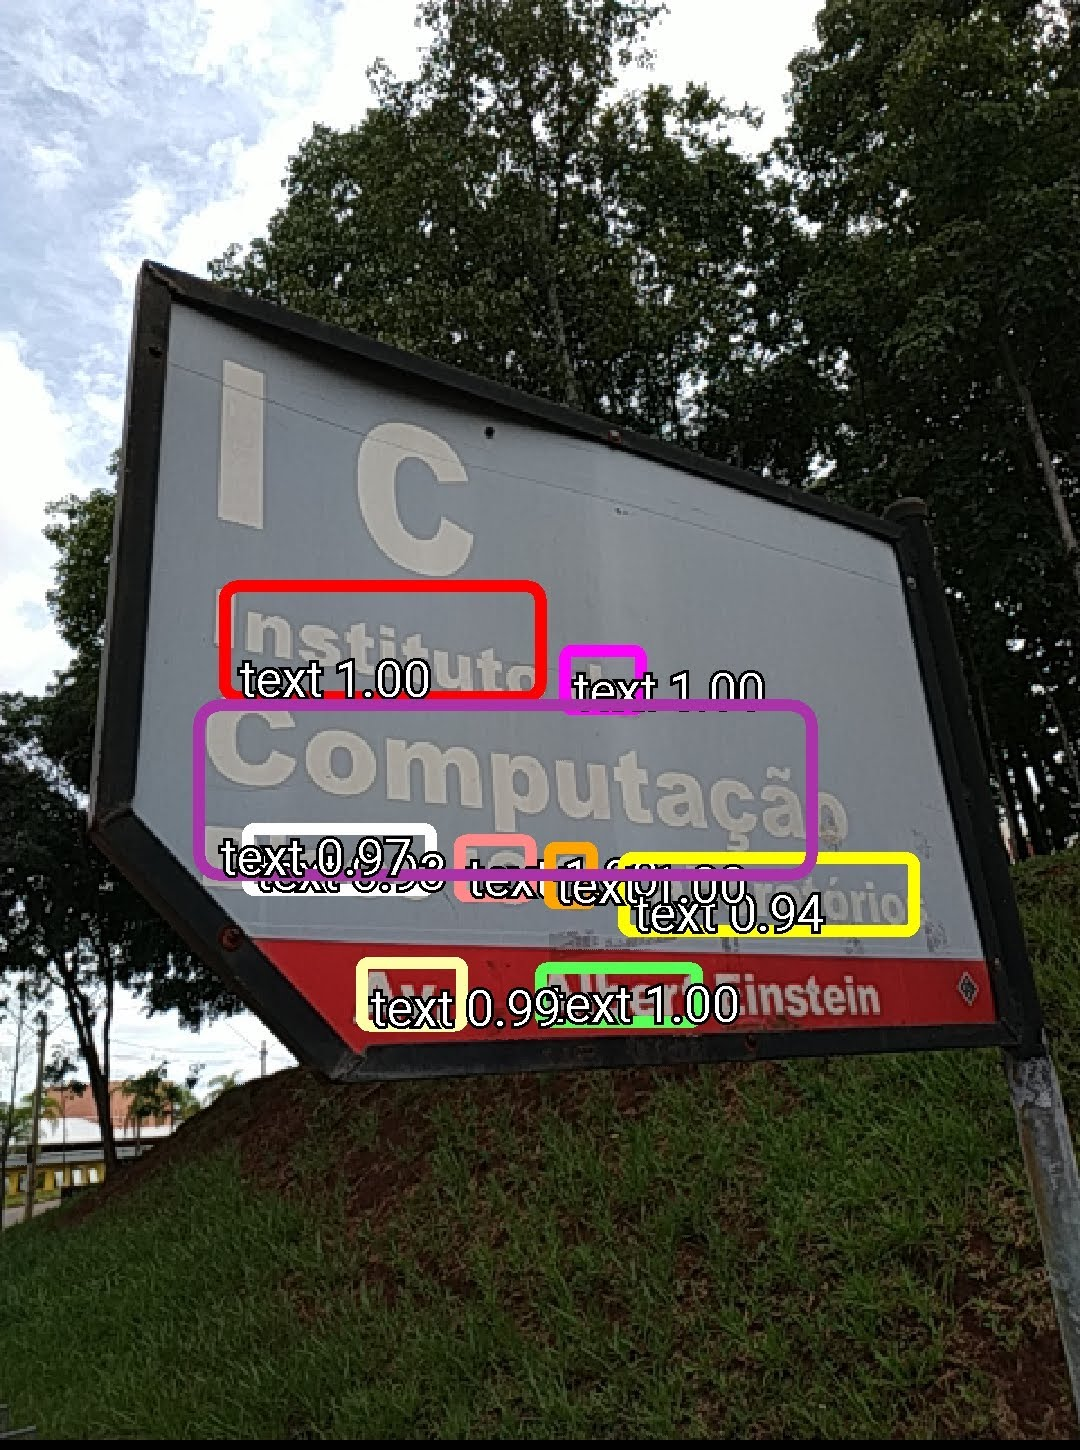
\includegraphics[width=0.49\textwidth]{Mobile/images/app28.jpg}

\caption{Example of scene text images captured with a perspective.}
\label{fig:ic-perspective}
\end{figure}
%%%%%%%%%%%%%%%%%%
Figure~\ref{fig:ic-perspective} shows the effect of the capturing angle of the texts in scene text images. As the system was only trained with horizontal aligned text, this kind of perspective lowers the system effectiveness.


\begin{figure}[h!]
\centering
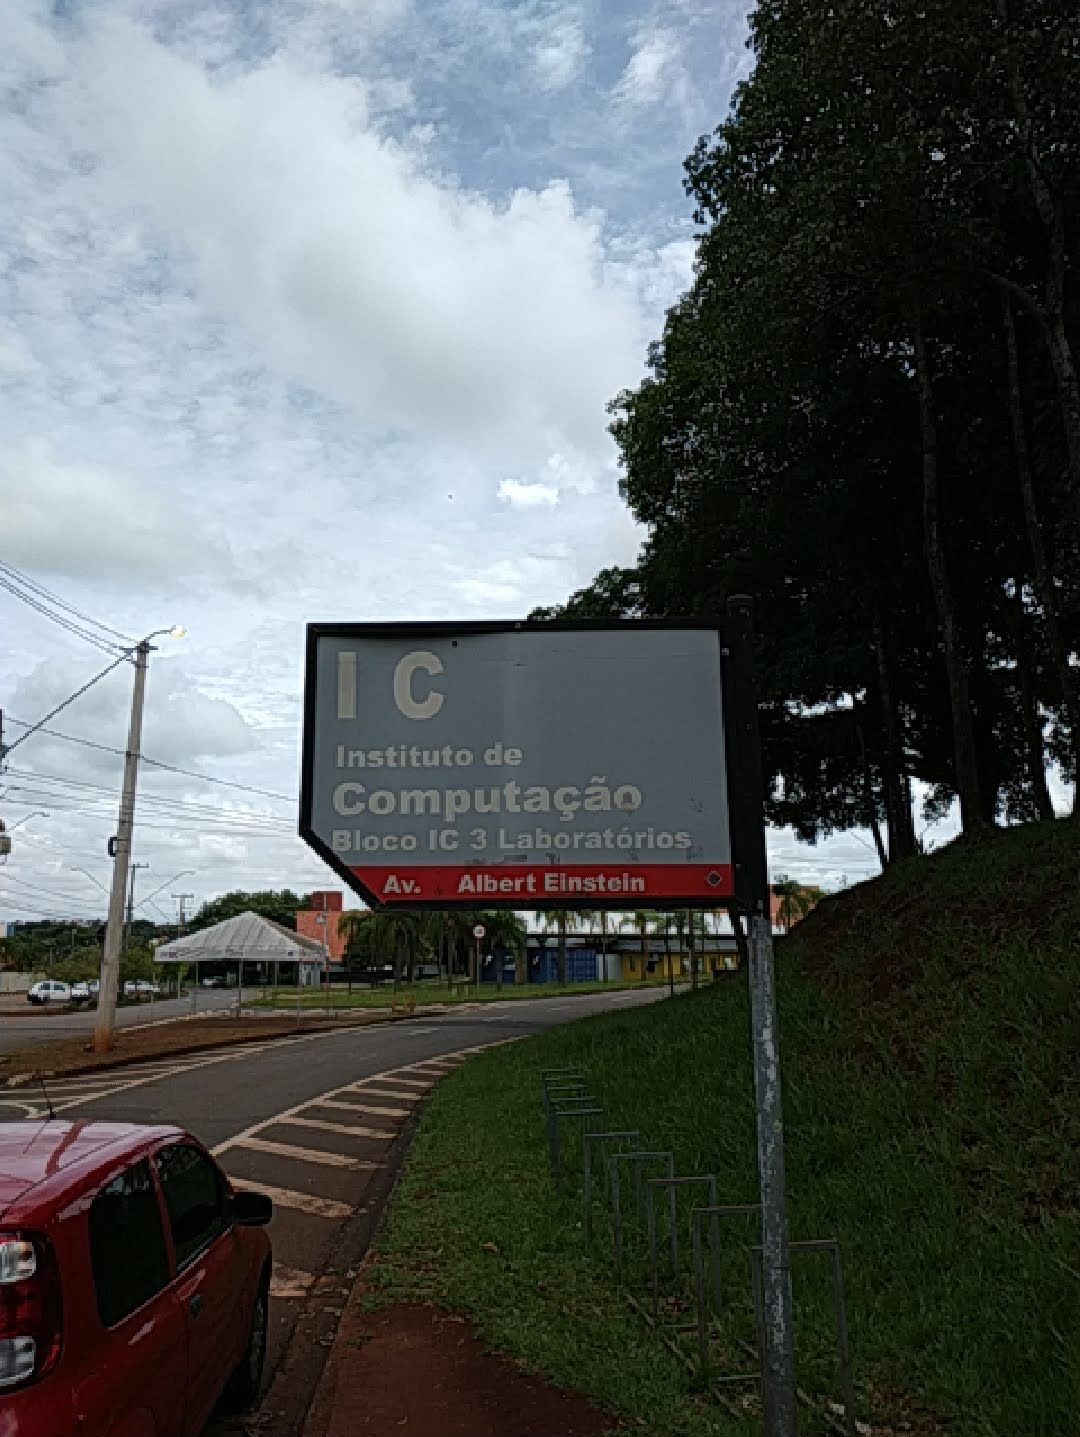
\includegraphics[width=0.49\textwidth]{Mobile/images/app24.jpg}
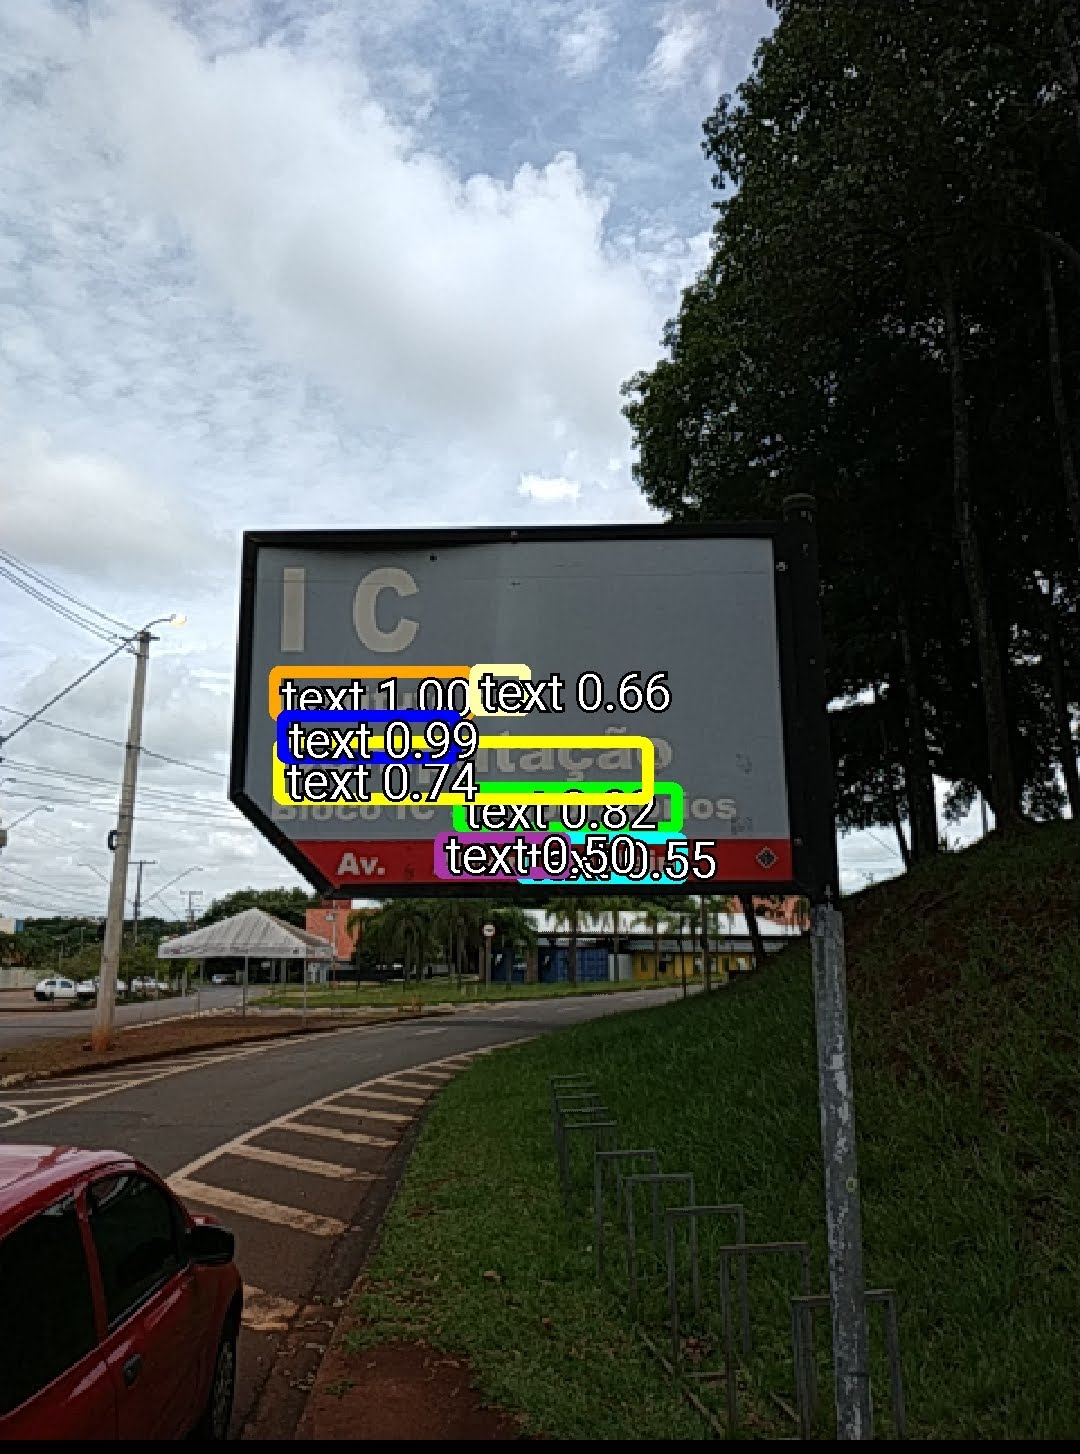
\includegraphics[width=0.49\textwidth]{Mobile/images/app25.jpg}

\vspace{1.5mm}

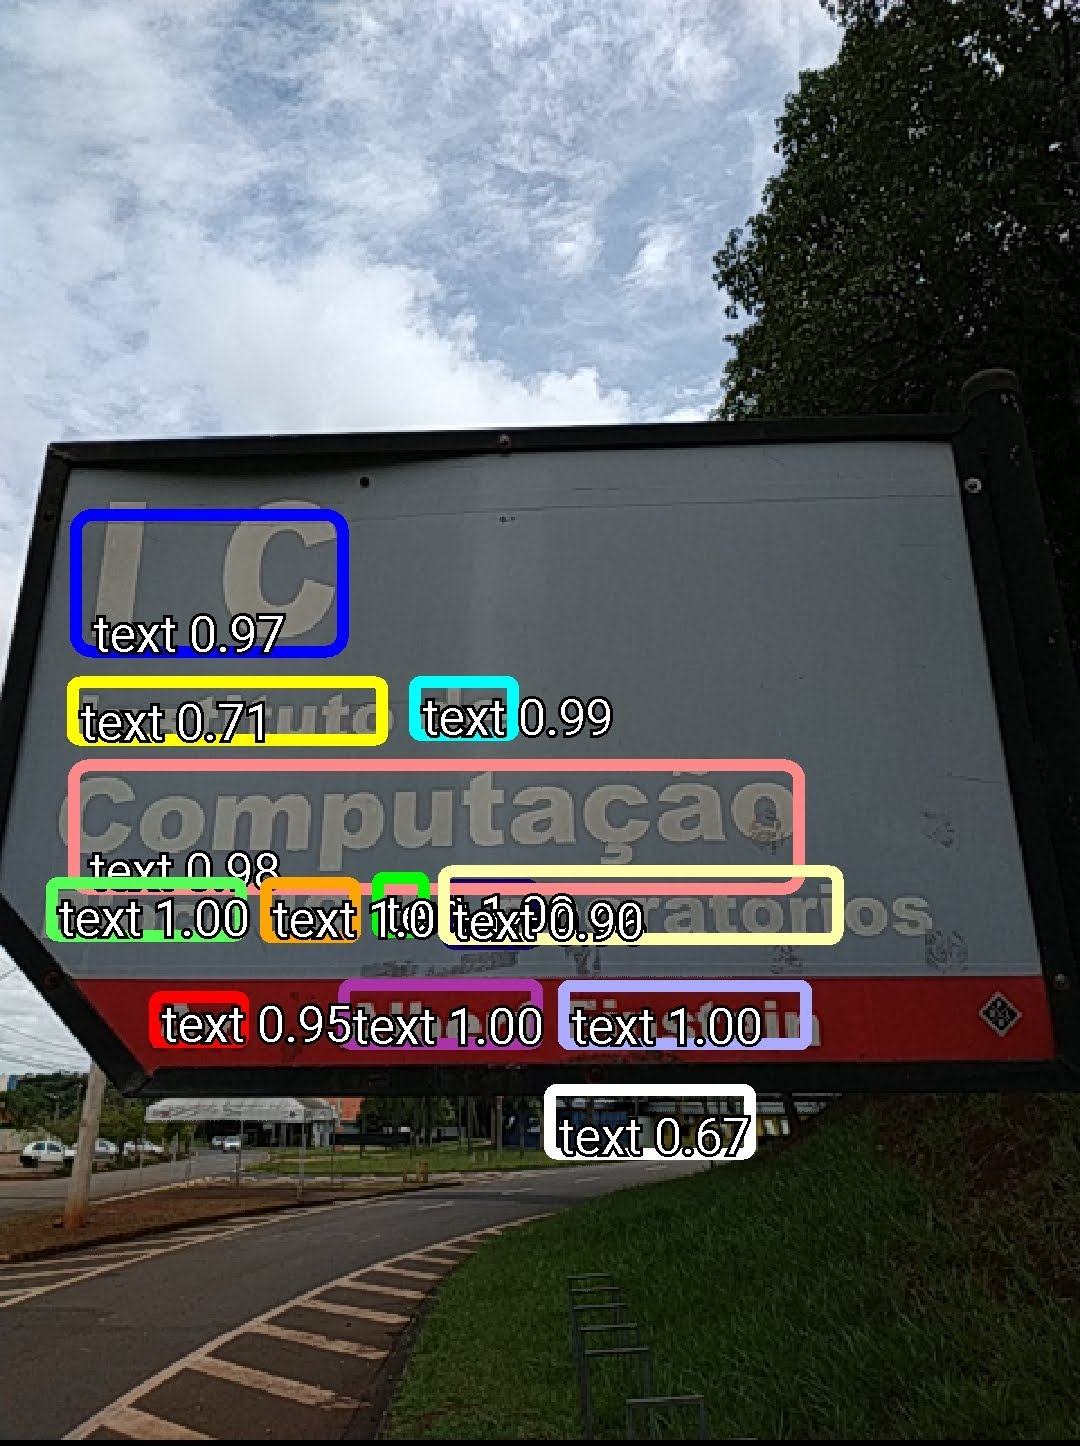
\includegraphics[width=0.49\textwidth]{Mobile/images/app23.jpg}
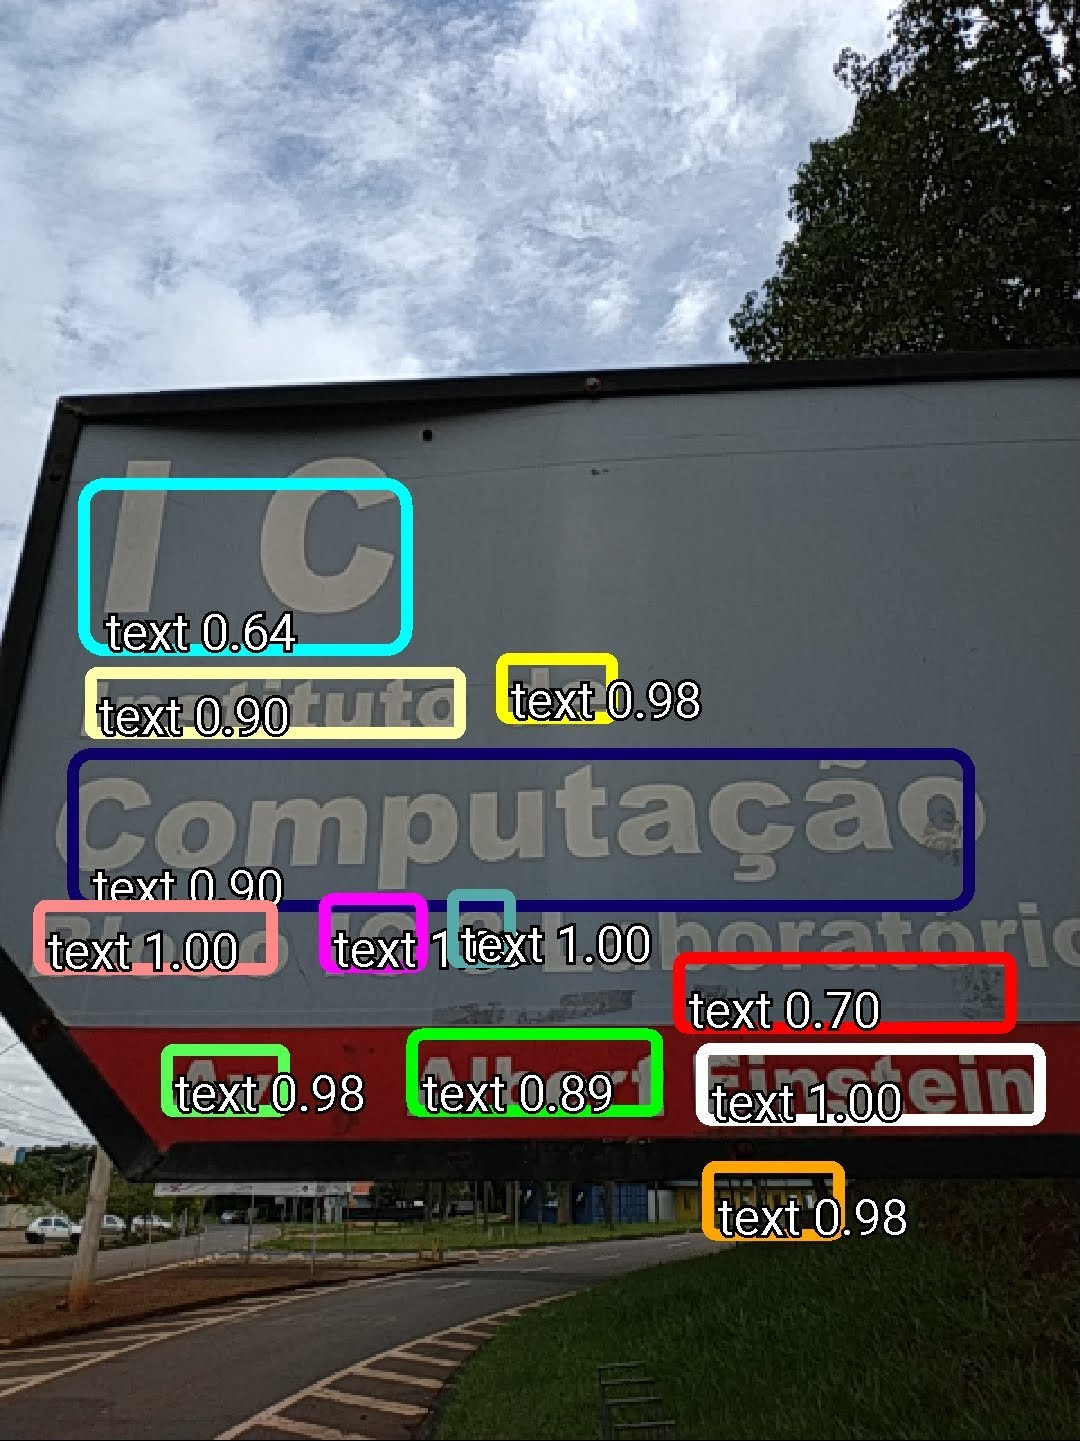
\includegraphics[width=0.49\textwidth]{Mobile/images/app26.jpg}


\caption{Example of scene text images captured with different zoom levels.}
\label{fig:ic-zoom}
\end{figure}
%%%%%%%%%%%%%%%%%
In Figure~\ref{fig:ic-zoom}, the effects of the size of the text on scene text images is shown. Images with smaller text (top left) are more difficult to detect, while image with medium to big text are easier and have better results, as shown in Figure~\ref{fig:sample_good}. 



\begin{figure}[h!]
\centering
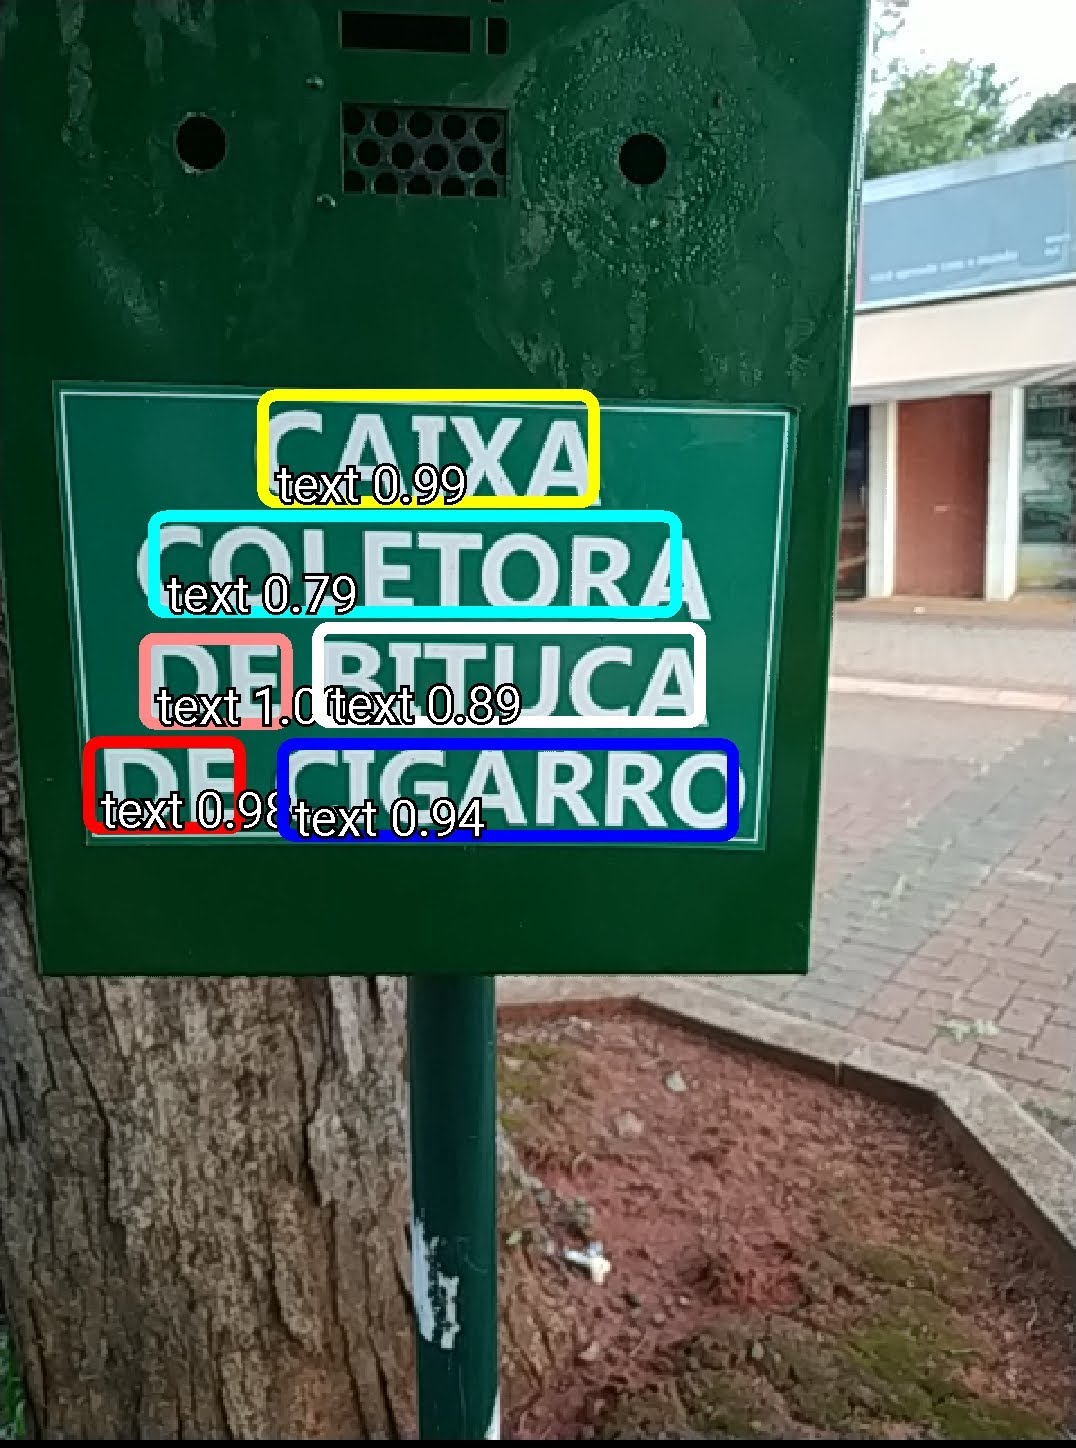
\includegraphics[width=0.49\textwidth]{Mobile/images/app03.jpg}
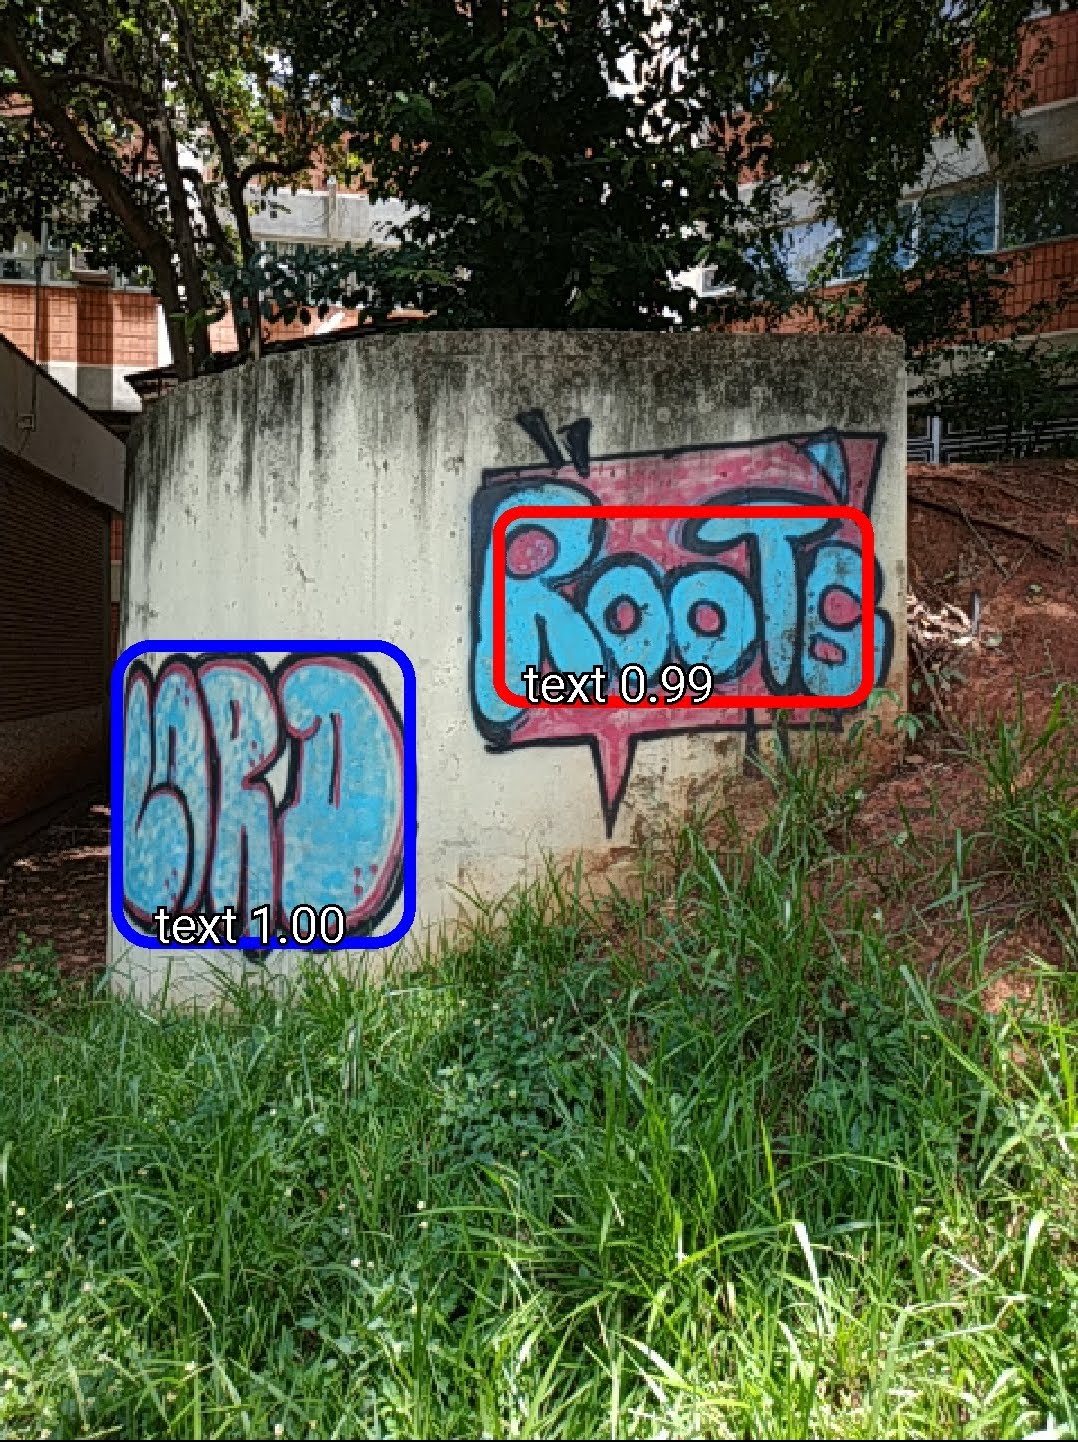
\includegraphics[width=0.49\textwidth]{Mobile/images/app09.jpg}

\vspace{1.5mm}

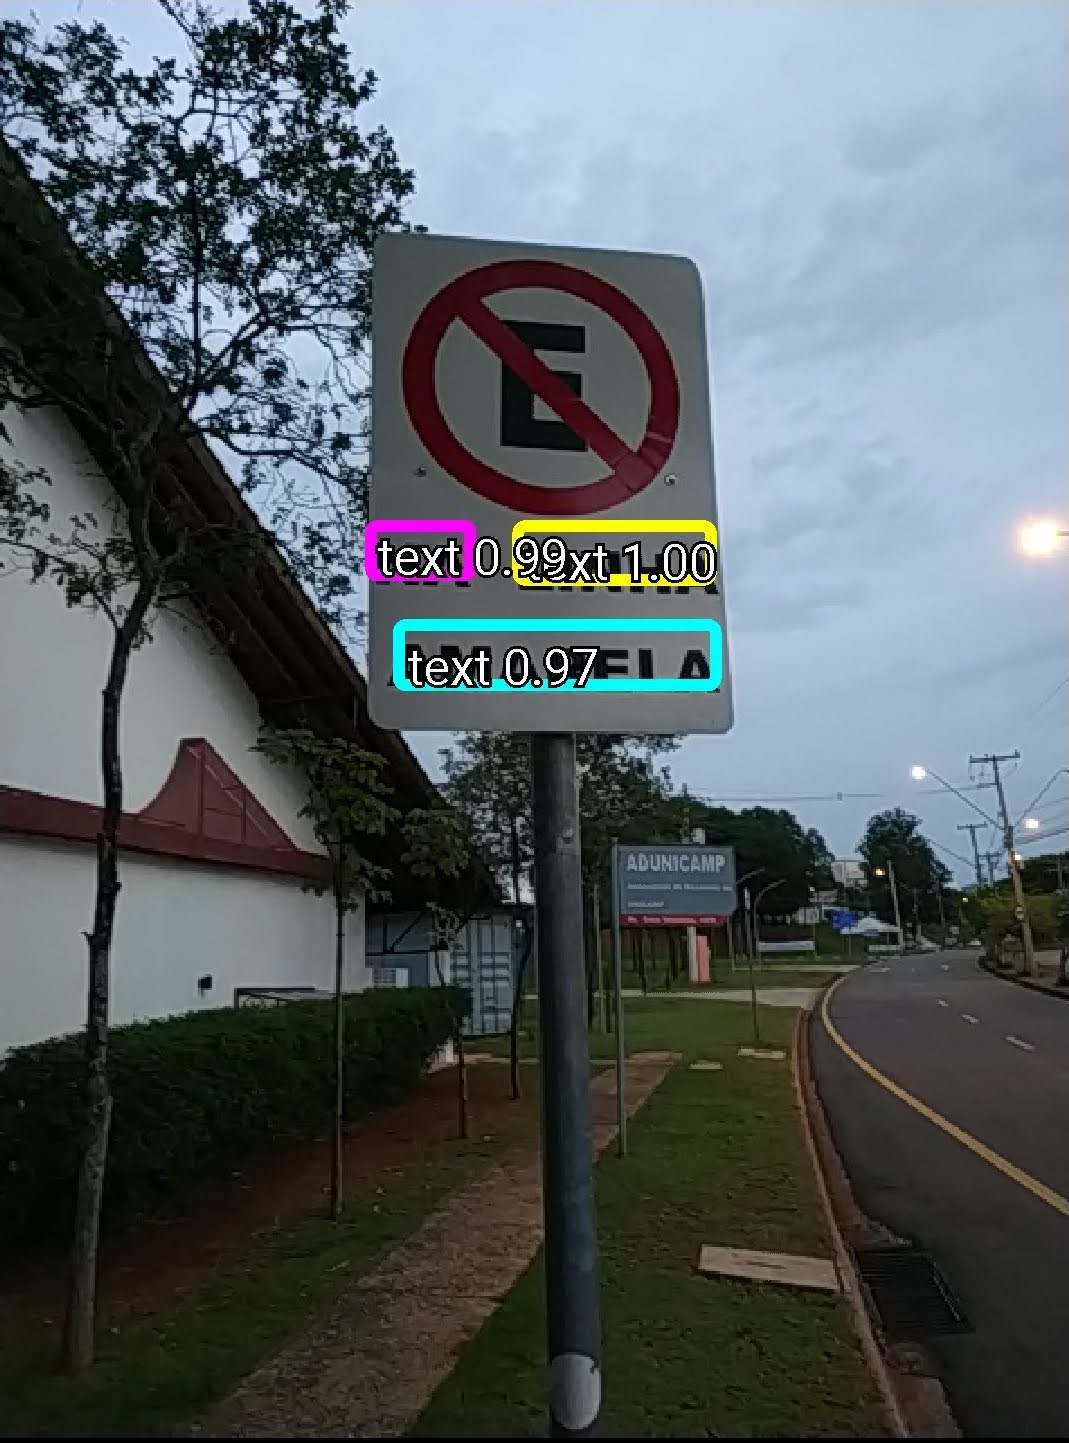
\includegraphics[width=0.49\textwidth]{Mobile/images/app07.jpg}
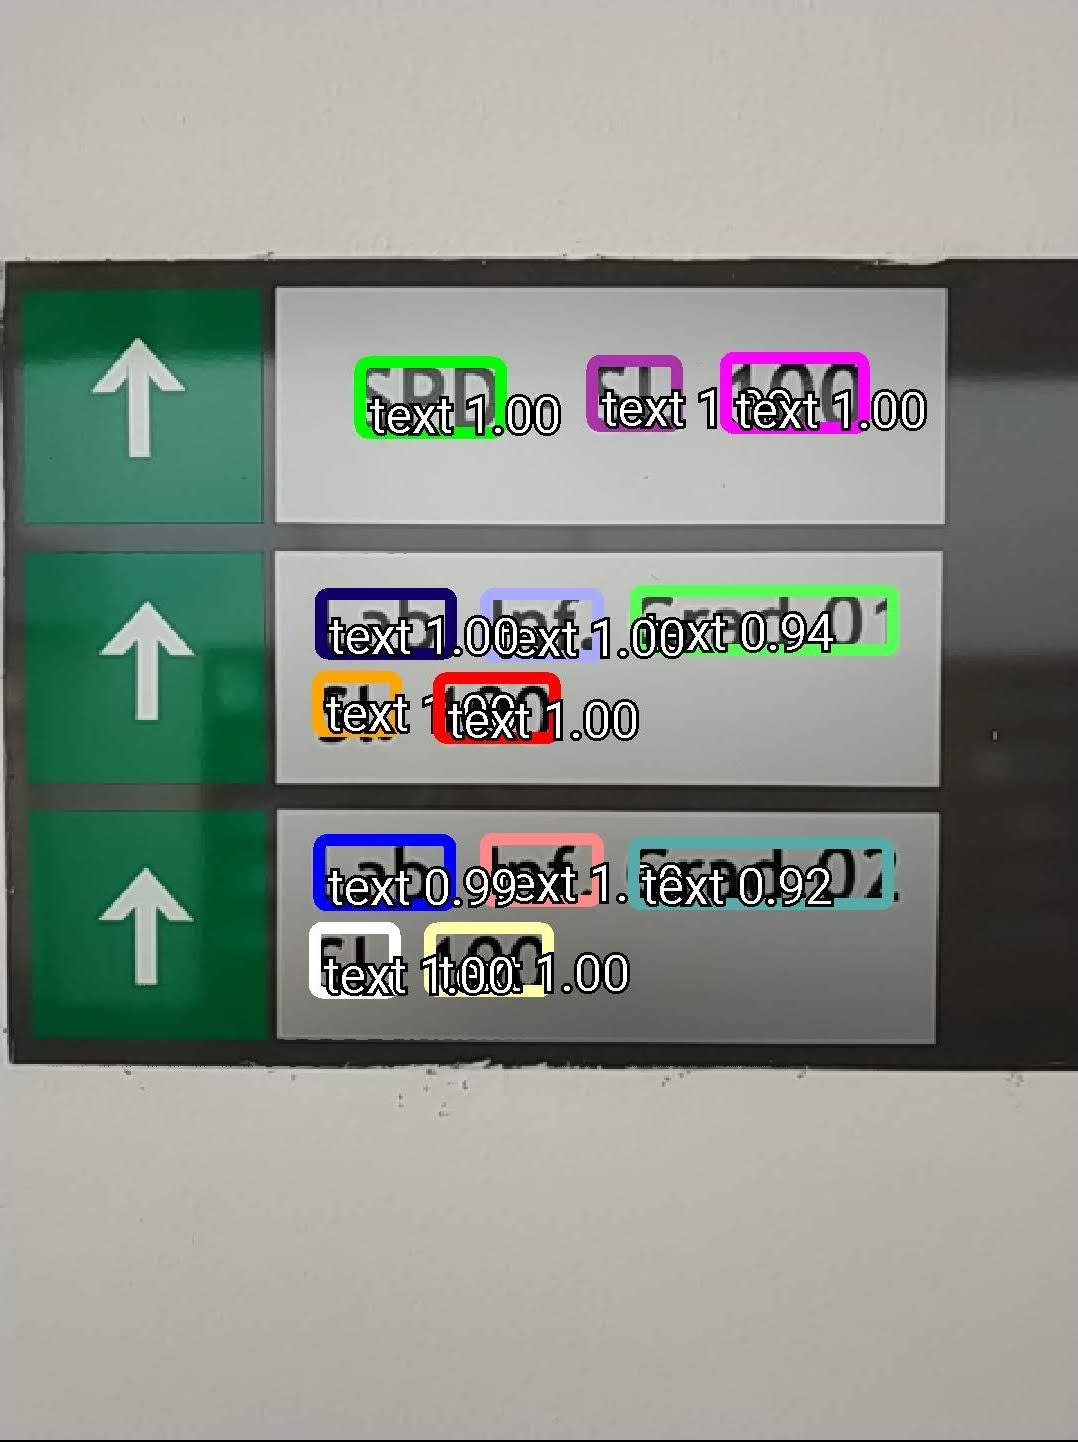
\includegraphics[width=0.49\textwidth]{Mobile/images/app11.jpg}


\caption{Example of scene text images with good results on our application.}
\label{fig:sample_good}
\end{figure}
%%%%%%%%%%%%%%%%%

Even though the system was not trained with handwritten text, the results of text detection on handwritten text, such as in Figure~\ref{fig:handwritten}, are very promising. Good detection results were obtained on handwritten text on a complex background (top left) and even on multilingual text (bottom left). 
\begin{figure}[h!]
\centering
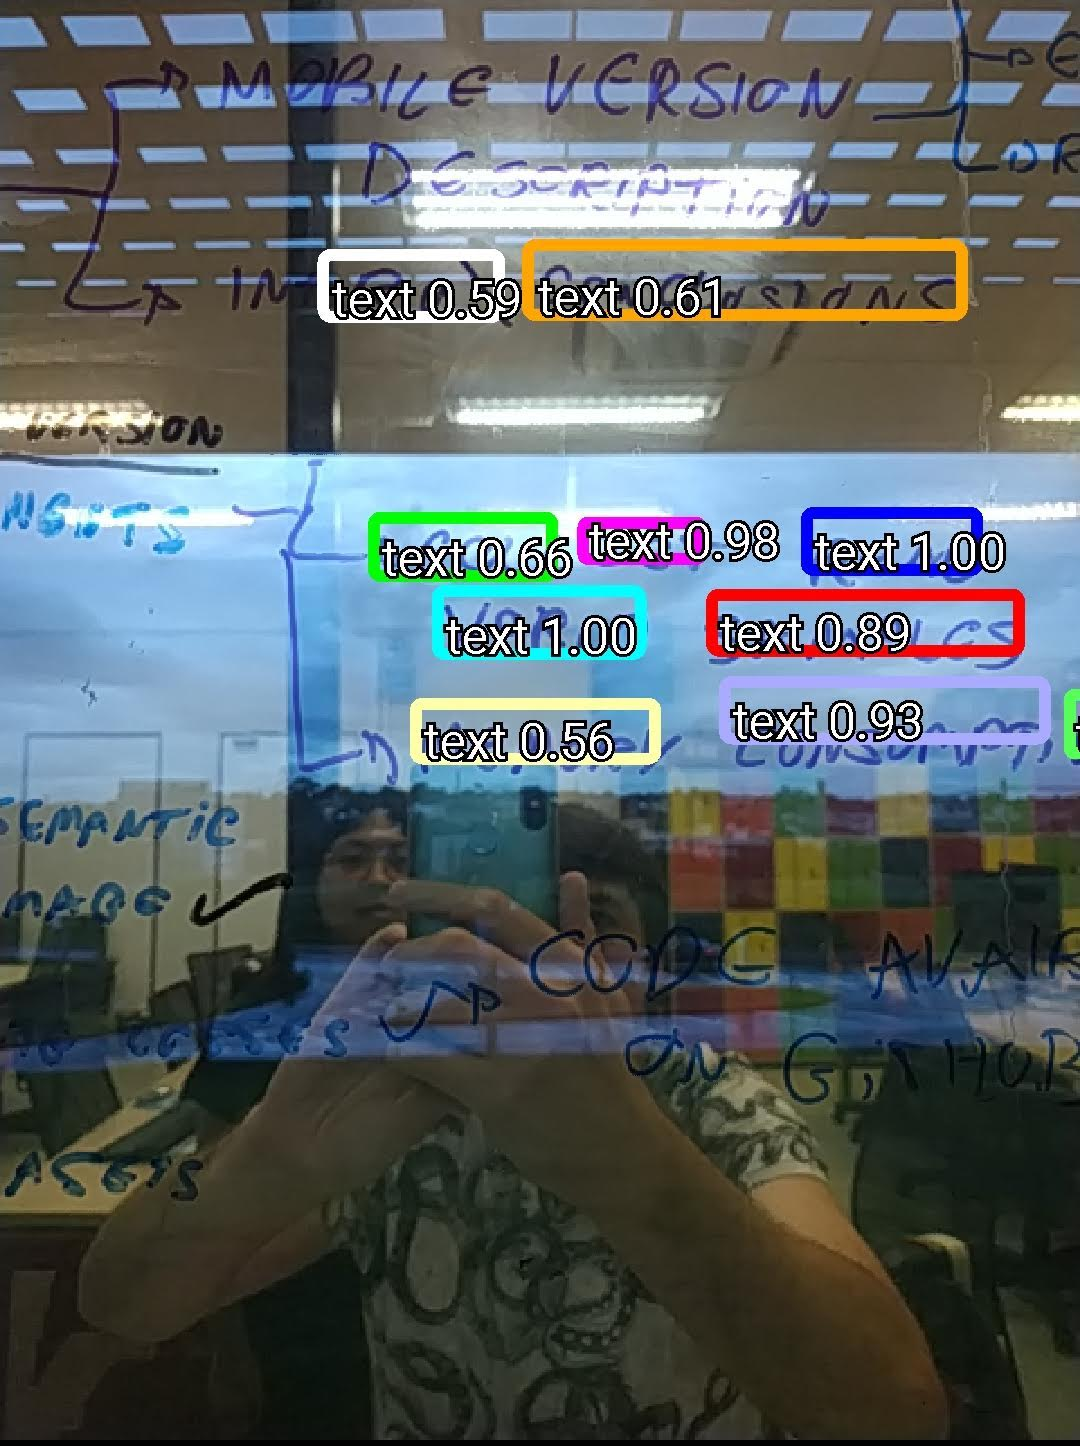
\includegraphics[width=0.49\textwidth]{Mobile/images/app22.jpg}
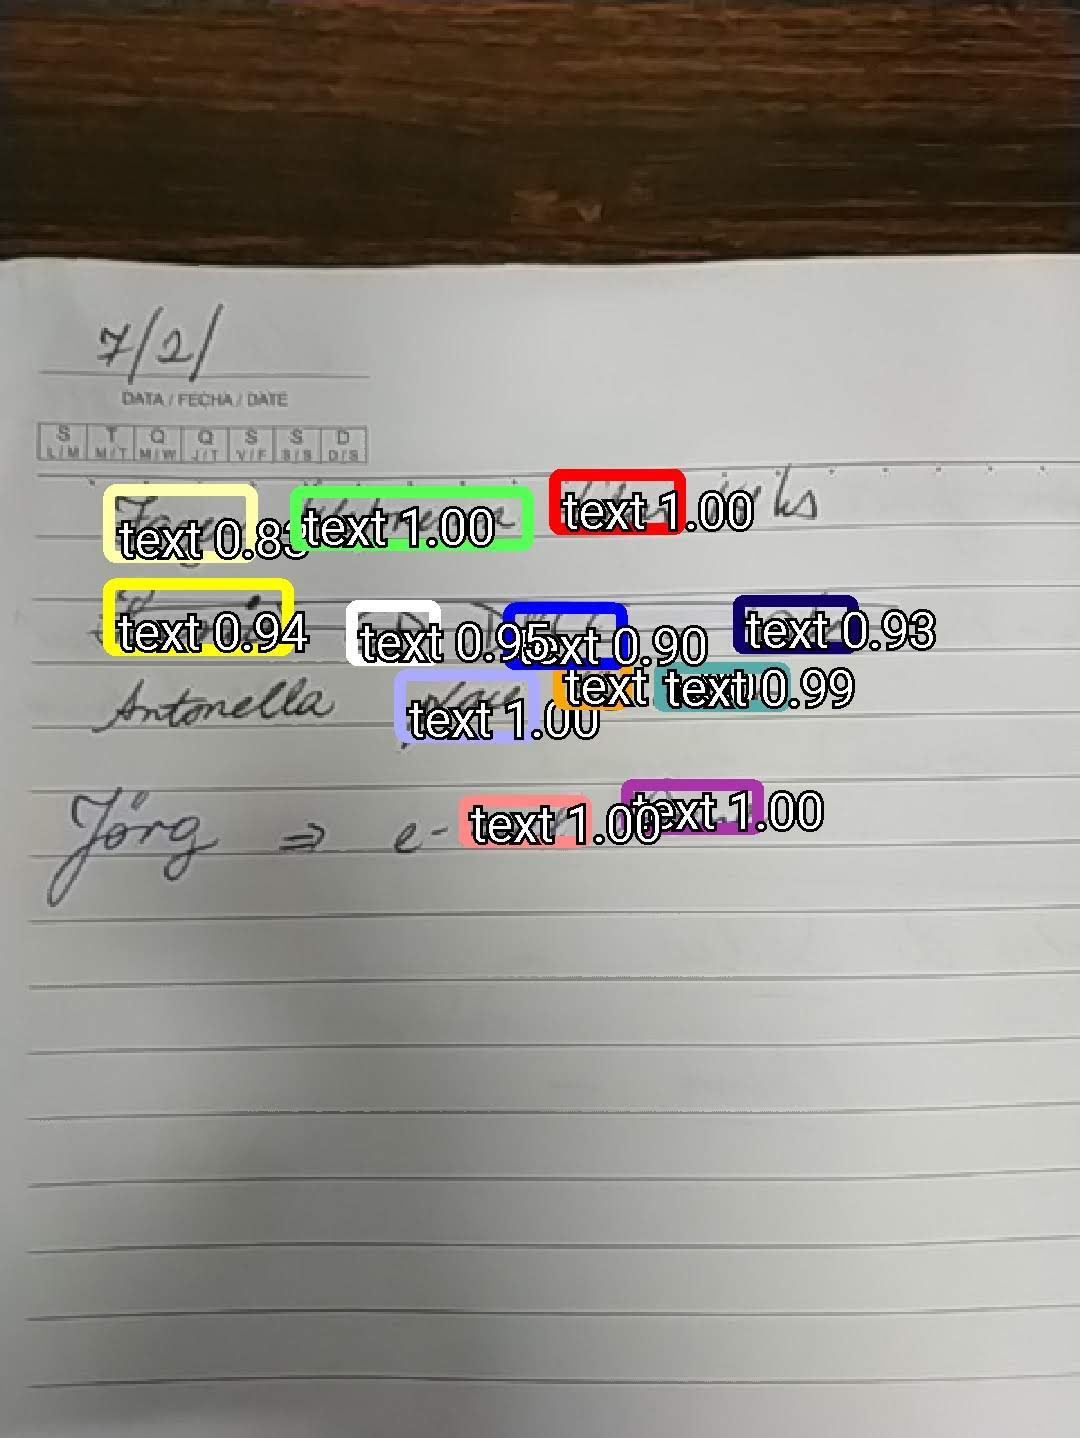
\includegraphics[width=0.49\textwidth]{Mobile/images/app31.jpg}

\vspace{1.5mm}

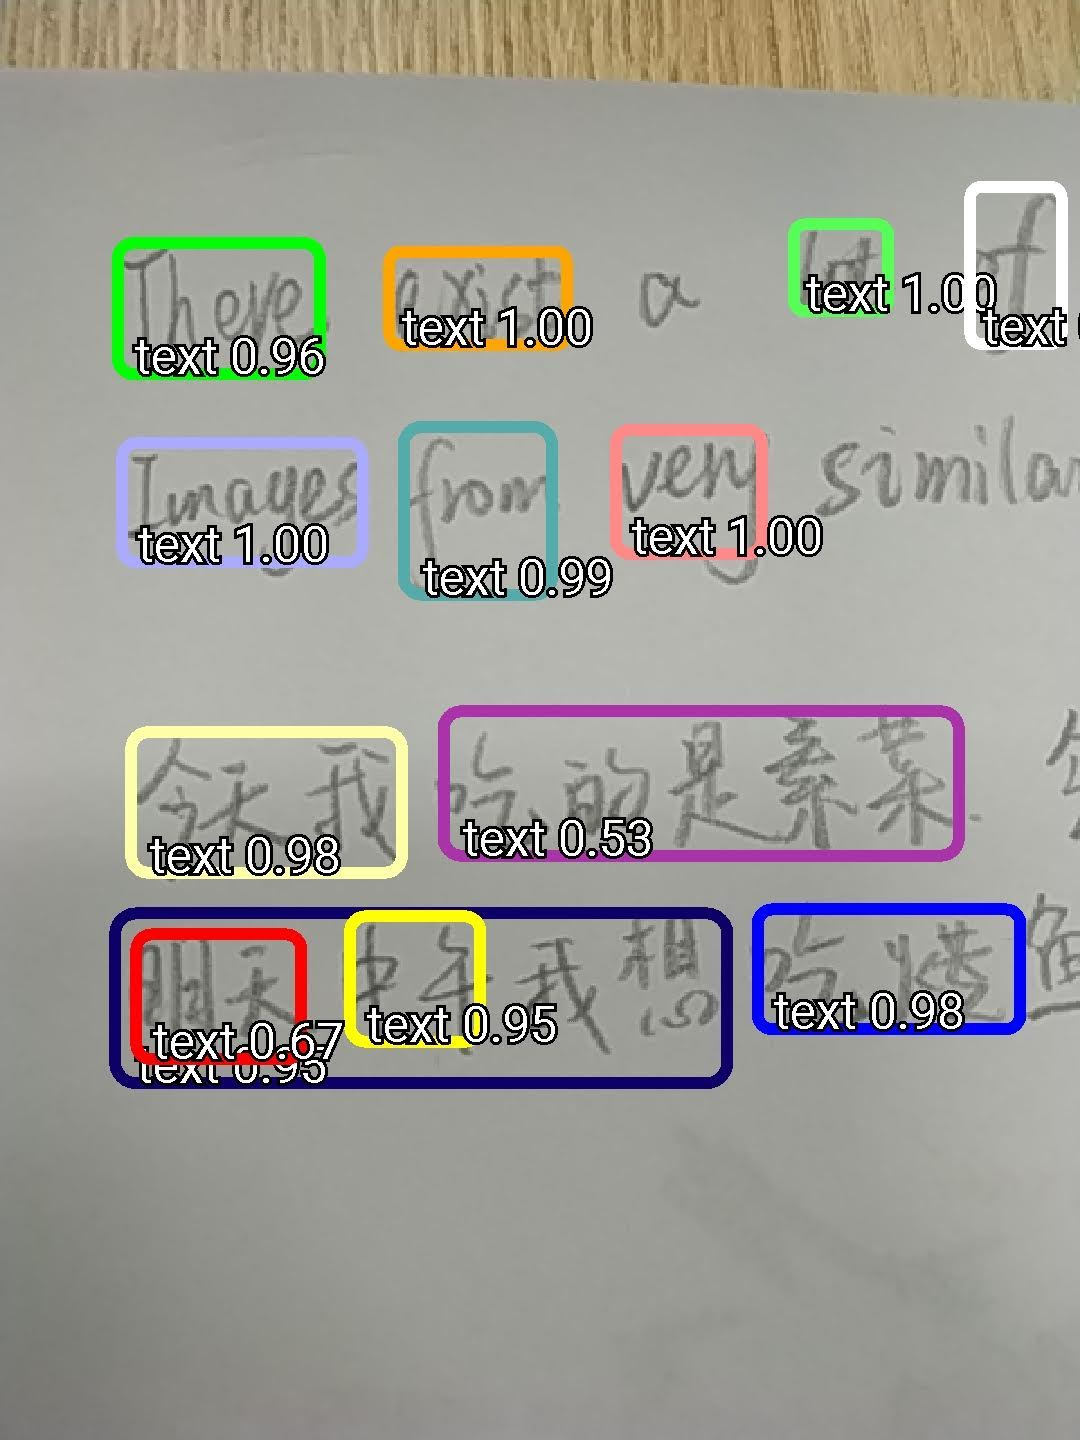
\includegraphics[width=0.49\textwidth]{Mobile/images/app17.jpg}
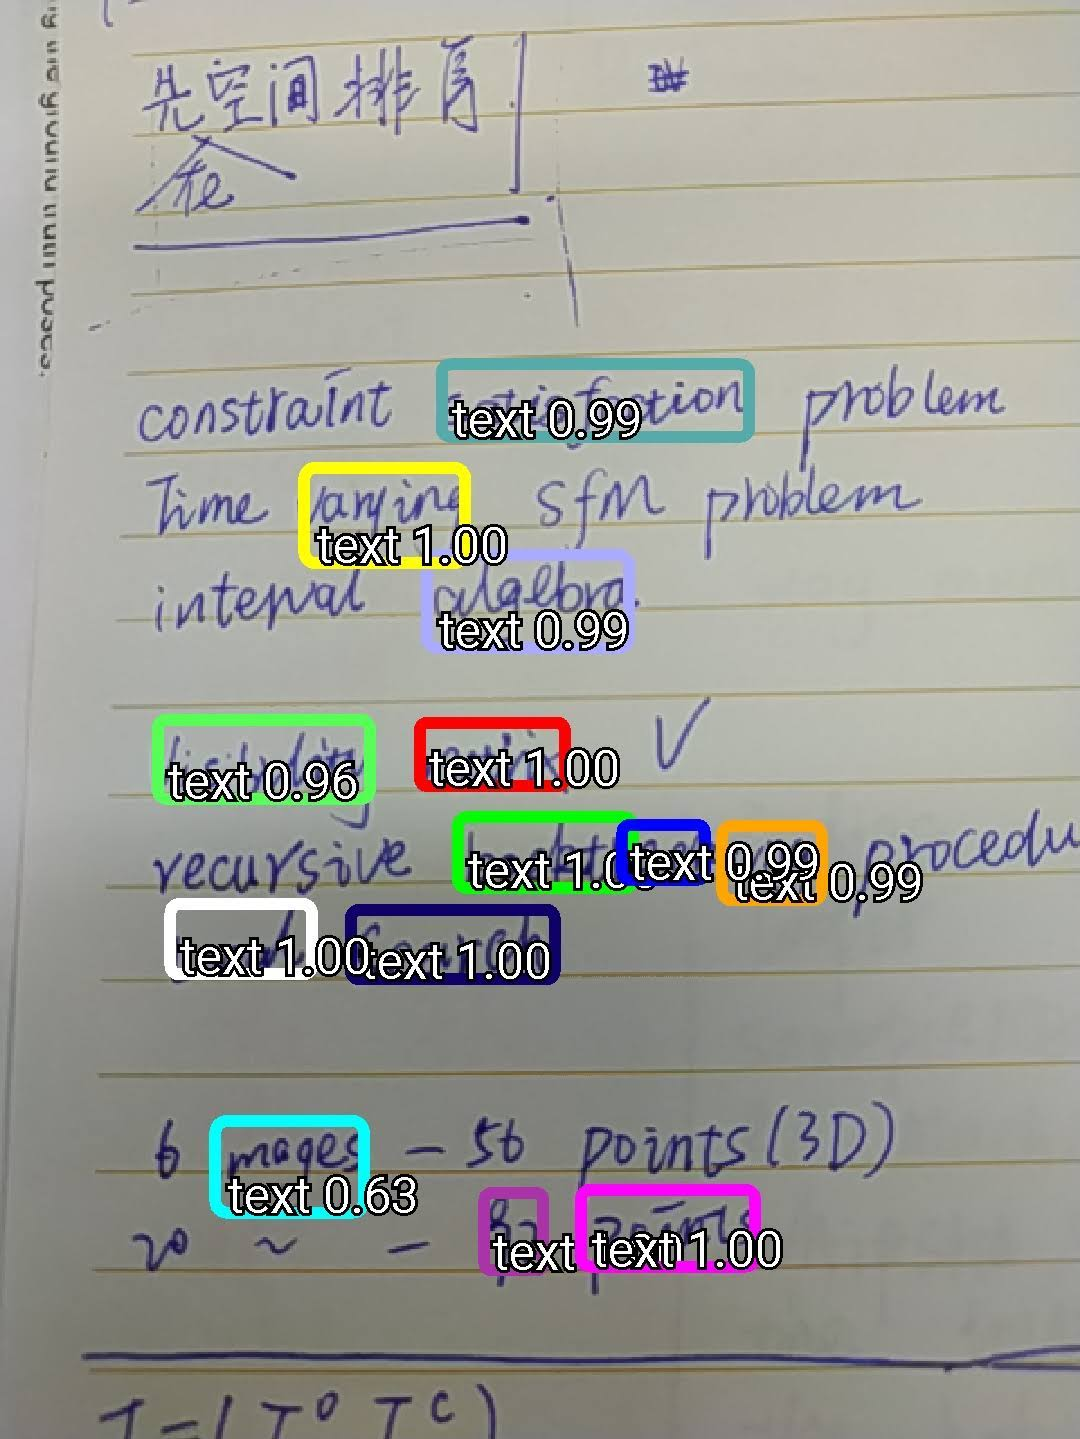
\includegraphics[width=0.49\textwidth]{Mobile/images/app18.jpg}


\caption{Example of handwritten text, with complex backgrounds and multilingual text.}
\label{fig:handwritten}
\end{figure}

%\begin{figure}[!t]
%	\centering
%	\hspace{0.1mm}
%	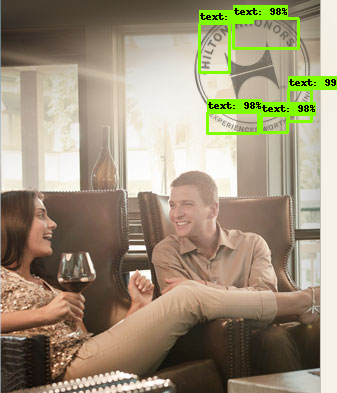
\includegraphics[height=0.27\columnwidth]{ICIP_frankenstein/figs/qualitative-results/icdar11-success-69.png}
%	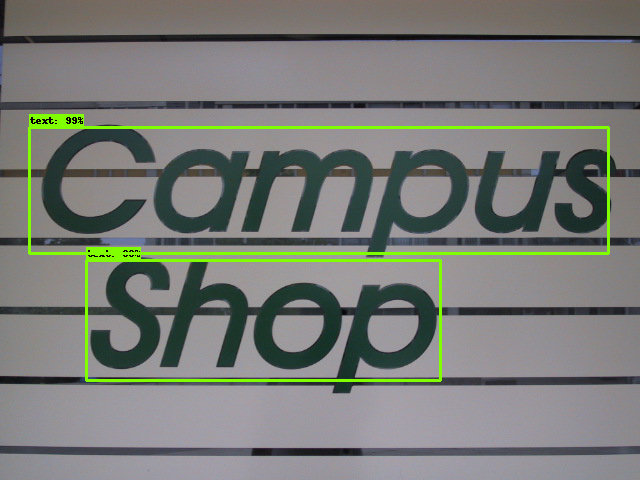
\includegraphics[height=0.27\columnwidth]{ICIP_frankenstein/figs/qualitative-results/icdar13-success-5.png}
%    \\ \vspace{0.5mm}
%	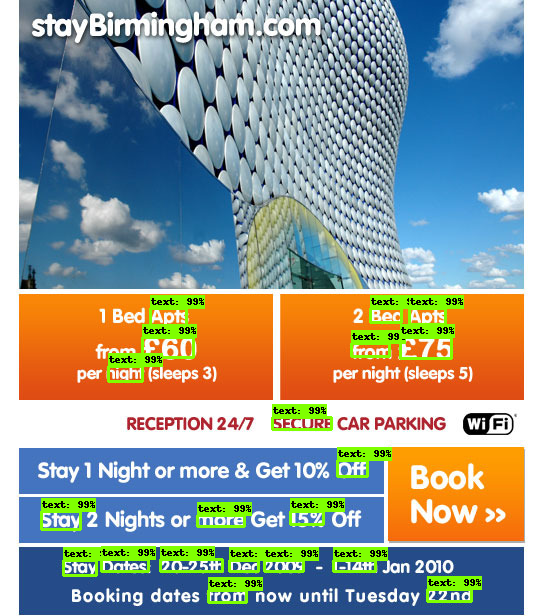
\includegraphics[height=0.27\columnwidth]{ICIP_frankenstein/figs/qualitative-results/icdar11-failure-10.png}
%	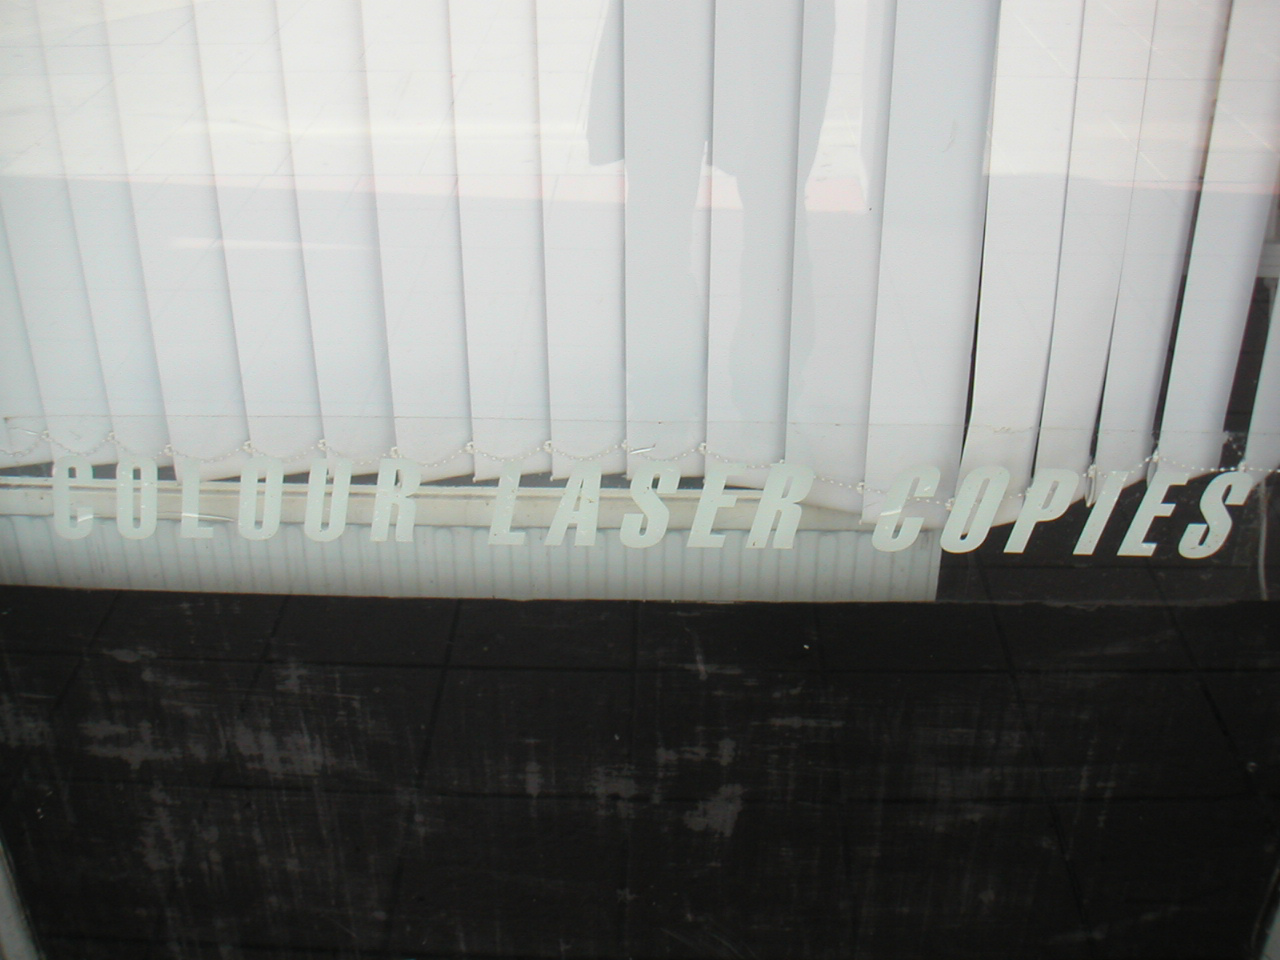
\includegraphics[height=0.27\columnwidth]{ICIP_frankenstein/figs/qualitative-results/icdar13-failure-185.png}
%	\caption{Examples of success (first line) and failure (second line) cases of the proposed approach for the ICDAR'11 (first column) and ICDAR'13 (second column) datasets.}
%	\label{fig:qualitative-results}
%\end{figure}



% Regarding the efficiency, in terms of processing time, the proposed method presented a very competitive results, taking only $0.09$ seconds per image, on average. This obtained processing time meets the results presented by the authors, which reported a computing speed about $0.02$ seconds per frame, considering an input image of $1,242 \times 375$ pixels.  For the disk usage performance, the lighter deep learning-based model was produced by SqueezeDet, with a size of $23.10$MB. On the other hand, the heaviest deep learning-based model was produced by SSTD network, with a size of $248.20$MB.
%
%\todo[inline]{Include the values for YOLOv3 in the table below}
%
% \begin{table}[!t]
%     \centering
%     \caption{Processing time per image, in seconds, for the evaluated deep learning-based methods.}
%     \label{tab:comparison-efficiency-time-proc-deep-methods-icdar11-icdar13}
%     \resizebox{\columnwidth}{!}{ 
%     \begin{tabular}{lrrr}
%         \topline
%         \headcol
%         \headcol \textbf{Methods} & \textbf{ICDAR'11} & \textbf{ICDAR'13} & \textbf{Average} \\
%         \midline
%         SSTD                      & $0.45$               & $0.55$               & $0.50$              \\ \hline
%         TextBoxes                 & $0.45$               & $0.53$               & $0.49$              \\ \hline
%         TextBoxes++               & $1.70$               & $1.87$               & $1.79$              \\ \hline
%         MobText           & $5.62$               & $4.32$               & $4.97$              \\ \hline
%         % YOLOv3                    & $6.84$               & $7.42$               & $7.13$              \\ \hline
%         % SqueezeDet                & $0.08$               & $0.09$               & $0.09$              \\
%       \bottomlinec
%     \end{tabular}}
% \end{table}
% %		
% \begin{table}[!t]
%     \centering
%     \caption{Comparison of efficiency, in terms of disk usage, among the evaluated deep learning-based methods.}
%     \label{tab:comparison-efficiency-disk-usage-deep-methods}
%     \begin{tabular}{lr}
%         \topline
%         \headcol \textbf{Methods} & \textbf{Disk usage (MB)}    \\
%         \midline
%         SSTD                      & $248.20$                    \\ \hline
%         TextBoxes                 & $95.10$                     \\ \hline
%         TextBoxes++               & $139.10$                    \\ \hline
%         MobText           & $37.00$                     \\ \hline
%         % YOLOv3                    & $246.30$                    \\ \hline
%         % SqueezeDet                & $23.10$                     \\
%       \bottomlinec
%     \end{tabular}
% \end{table}
